% hello
\documentclass{article}

\usepackage[utf8]{inputenc}
\usepackage{graphicx}
\usepackage[dvipsnames]{xcolor}
\usepackage{csquotes}
\usepackage{hyperref}
\usepackage{tabularx}
\usepackage{booktabs}
\usepackage{pdfpages}
\usepackage{caption,geometry}
\usepackage[toc,page]{appendix}
\newcommand\myshade{85}
\colorlet{mylinkcolor}{violet}
\colorlet{mycitecolor}{YellowOrange}
\colorlet{myurlcolor}{Aquamarine}

\hypersetup{
  linkcolor  = mylinkcolor!\myshade!black,
  citecolor  = mycitecolor!\myshade!black,
  urlcolor   = myurlcolor!\myshade!black,
  colorlinks = true,
}

\usepackage[acronym]{glossaries}

\usepackage{listings}
\lstset{
    frame=Trbl,
    numbers=left,
    breaklines=true,
    basicstyle=\ttfamily,
    postbreak=\mbox{\textcolor{red}{$\hookrightarrow$}\space}
}

\usepackage[maxnames=3,style=authoryear,natbib=true]{biblatex}
\addbibresource{./references.bib}
% \bibliographystyle{unsrtnat}
% \setcitestyle{authoryear}


\newglossary[bsg]{bus}{bsd}{bsn}{Bussiness glossary}
\newglossary[dmg]{dm}{dmd}{dmn}{Data mining glossary}

\graphicspath{ {../images/} }

\DeclareUnicodeCharacter{2008}{-}% support older LaTeX versions
\DeclareUnicodeCharacter{2003}{ }% support older LaTeX versions

\let\oldautoref\autoref
\renewcommand{\autoref}[1]{(\oldautoref{#1})}
\newcommand{\autorefsub}[2]{(\oldautoref{#1}, #2)}
\newcommand{\gmt}{\acrshort{gmt}}
\newcommand{\firstvis}{first-visit data }
\newcommand{\secondvis}{second-visit data }

\newcommand{\uu}{Utrecht University}
\newcommand{\flup}{\gls{d:flup} }
\newcommand{\simon}{\gls{d:simon} }
\newcommand{\dpaper}{the \flup paper }
\newcommand{\Dpaper}{The \flup paper }
\newcommand{\spaper}{the \simon paper }

\newcommand{\MyTitle}[1]{
    \title{
    {#1}\\
    {\large Utrecht University}\\
    }
    \author{Mike Vink}
    \date{ \today }
    \maketitle
}
\newcommand{\f}[3]{%
\begin{figure}[htpb]
    \includegraphics[width=\textwidth]{#1}
    \caption{#2}
    \label{#3}
\end{figure}
}

\newcommand{\fptable}[5]{%

\newgeometry{scale=1}
\thispagestyle{empty}

\begin{table}
{%
    \centering
    \includegraphics[scale=.7]{#1}
    \captionsetup{width=0.8\linewidth}
    \captionof{table}{\textbf{#3} #4}
    \par
    \label{#5}
}
\end{table}

\restoregeometry
}

\newcommand{\fpfig}[5]{%

\newgeometry{scale=1}
\thispagestyle{empty}

\begin{figure}
{%
    \centering
    \includegraphics[scale=.7]{#1}
    \captionsetup{width=0.8\linewidth}
    \captionof{figure}{\textbf{#3} #4}
    \par
    \label{#5}
}
\end{figure}

\restoregeometry
}



\makeglossaries
\newglossaryentry{bu:rnaVirus}
{
    type=bus,
    name=ribonucleic acid virus(es),
    description={An \acrshort{rna} virus is a virus that has \acrshort{rna} as
    its genetic material. Inside a host cell this material is used to generate
    new virusses. Notable human diseases caused by RNA viruses include the
    common cold and influenza}
}
\newglossaryentry{bu:antigen}
{
    type=bus,
    name=antigen,
    description={In immunology, an antigen is a molecule or molecular
    structure, such as \acrshort{ha} and \acrshort{na}, that can be bound by an
    antigen-specific \gls{bu:antibody} or immune cell receptor.  The presence of
    antigens in the body normally triggers an immune response
    }
}
\newglossaryentry{bu:glycoprotein}
{
    type=bus,
    name=glycoprotein,
    description={Glycoproteins are molecules that comprise protein and
    carbohydrate chains. Many viruses have external glycoproteins that
    help them enter bodily cells, but can also serve to be important
    therapeutic or preventative targets}
}
\newglossaryentry{bu:mutation}
{
    type=bus,
    name=mutation,
    description={Mutation of genetic material occurs thanks to its chemical
    instability. The encoded protein molecules can have single amino acid
    (protein building block) change (minor, but still in many cases significant
    change leading to disease) or wide-range amino acid changes}
}
\newglossaryentry{bu:tiv}
{
    type=bus,
    name=TIV,
    description={
        An inactivated trivalent vaccine is a vaccine consisting of \gls{bu:antigen}ic virus particles from viruses that have been grown in culture and then killed to destroy disease producing capacity.
        In practice vaccines of three main types of influenza were used, hence trivalent
    },
    first={inactivated trivalent vaccines (TIV)}
}
\newglossaryentry{bu:antibody}
{
    type=bus,
    name=antibody,
    description={ Protein used by the immune system to identify and neutralize foreign objects such as pathogenic bacteria     and viruses.
    The antibody recognizes a unique molecule of the pathogen, called an \gls{bu:antigen}}
}
\newglossaryentry{bu:titer}
{
    type=bus,
    name=titer,
    description={
    Titer is a way of expressing concentration.
    Titer testing employs serial dilution to obtain approximate quantitative information from an analytical procedure that inherently only evaluates as positive or negative.
    The titer corresponds to the highest dilution factor that still yields a positive reading
    }
}
\newglossaryentry{bu:tcell}
{
    type=bus,
    name=T-cell,
    description={
        A T cell is a type of \gls{bu:lymphocyte}.
        T cells are one of the important white blood cells of the immune system and play a central role in the adaptive immune response, for example generating antibodies against influenza.
        Groups of specific, T cell subtypes have a variety of important functions in controlling and shaping the adaptive immune response
    }
}
\newglossaryentry{bu:lymphocyte}
{
    type=bus,
    name=lymphocyte,
    description={
        A lymphocyte is a type of white blood cell in the immune system of jawed vertebrates.
        Lymphocytes include \gls{bu:tcell}, and \gls{bu:bcell}.
        These cells work together in the adaptive immune response to generate antibodies against influenza
    }
}
\newglossaryentry{bu:cd8pos}
{
    type=bus,
    name=CD8+ T-cell,
    description={
        A cytotoxic T cell (also known as CD8+ T-cell) is a \gls{bu:tcell} that kills cancer cells, cells that are infected (particularly with viruses), or cells that are damaged in other ways.
        It does so by recognizing specific part of \gls{bu:antigen} and then starting a process that kills the targetted cell
    }
}
\newglossaryentry{bu:cd4pos}
{
    type=bus,
    name=CD4+ T-cell,
    description={
        The T helper cells, also known as CD4+ cells, "help" the activity of other immune cells by releasing \gls{bu:cytokine}s.
        These cells help to polarize the immune response into the appropriate kind depending on the nature of the immunological insult (e.g. virus vs. bacterium)
    }
}
\newglossaryentry{bu:cytokine}
{
    type=bus,
    name=cytokine,
    description={
        Cytokines are a broad and loose category of small proteins important in cell signaling that bind to receptor protein on the outside of (immune) cells to fulfill their signal function
    }
}
\newglossaryentry{bu:pbmc}
{
    type=bus,
    name=PBMC,
    description={
        A peripheral blood mononuclear cell is any peripheral blood cell having a round nucleus.
        These cells consist of \gls{bu:lymphocyte} and \gls{bu:monocyte}s
    },
    first={peripheral blood mononuclear cell (PBMC)}
}
\newglossaryentry{bu:bcell}
{
    type=bus,
    name=B-cell,
    description={
        B-cells produce antibody molecules; however, these antibodies are not secreted.
        Rather, they are presented on the outside of the cell where they serve as a part of B-cell receptors.
        When a B-cell is activated by an antigen, it proliferates and differentiates into an antibody-secreting effector cell, known as a plasmablast or plasma cell
    }
}
\newglossaryentry{bu:monocyte}
{
    type=bus,
    name=monocyte,
    description={
        Monocytes are a type of white blood cell.
        Monocytes and their macrophage and dendritic cell progeny serve three main functions in the immune system.
        These are phagocytosis, antigen presentation, and cytokine production.
        Phagocytosis is the process of uptake of microbes and particles followed by digestion and destruction of this material
    }
}
\newglossaryentry{bu:hai}
{
    type=bus,
    name=HAI,
    description={
        The \acrlong{ha} inhibition assay is used to measure the \gls{bu:titer} of \gls{bu:antibody} against a strain of influenza virus present in the serum.
        Antibody levels are measured before vaccination and 28 days after.
        The antibody levels are used to compute the seroprotection and seroconversion criteria
    },
    first={\acrlong{ha} inhibition assay (HAI)}
}
\newglossaryentry{bu:cmv}
{
    type=bus,
    name=CMV,
    description={
        Cytomegalovirus (CMV) is a common herpesvirus found in humans.
        Like other herpesviruses, it is a life-long infection that remains in a latent state inside the human body, until it is 'reactivated' by appropriate conditions.
        Thought to accelerate aging of the immune system and thereby impairing influenza vaccine response  \citep{van_den_Berg_2019}
    },
    first={cytomegalovirus (CMV)}
}
\newglossaryentry{bu:ebv}
{
    type=bus,
    name=EBV,
    description={
        The Epstein–Barr virus (EBV), is one of the nine known human herpesvirus types in the herpes family, and is one of the most common viruses in humans.
    },
    first={Epstein-Barr virus (EBV)}
}
\newglossaryentry{bu:seropc}
{
    type=bus,
    name=seroconversion and seroprotection,
    description={
        A vaccine is considered succesful if the recipient seroconverted (4-fold or greater rise in antibody against virus after vaccination) and were seroprotected (\acrshort{gmt} \(\ge\) 40) after vaccination.
    }
}
\newglossaryentry{bu:stat}
{
    type=bus,
    name=STAT,
    description={
        A vaccine is considered succesful if the recipient seroconverted (4-fold or greater rise in antibody against virus after vaccination) and were seroprotected (\acrshort{gmt} \(\ge\) 40) after vaccination.
    },
    first={signal transducers and activators of transcription (STAT)}
}



\newglossaryentry{d:model}
{
    type=dm,
    name=model,
    description={model is a model}
}
\newglossaryentry{d:flup}
{
    type=dm,
    name=FluPrint,
    description={Data used in this work}
}
\newglossaryentry{d:simon}
{
    type=dm,
    name=SIMON,
    description={Follow up study used in this work}
}

\newacronym{ha}{HA}{hemagglutinin}
\newacronym{na}{NA}{neuraminidase}
\newacronym{rna}{RNA}{ribonucleic acid}


\begin{document}
\MyTitle{Change in immune cell signaling upon repeat vaccination: a data exploration using the FluPrint database}
\tableofcontents
\newpage
\printglossary[type=bus]
\newpage
\printglossary[type=dm]
\newpage
\printglossary[type=\acronymtype]
\newpage


\section{Background}

Influenza viruses are enveloped \gls{bu:rnaVirus} (\acrshort{rna} virus(es)) and are divided into three types on the basis of \gls{bu:antigen}ic differences of internal structural proteins \citep{fdaGuidanceIndustryClinical2007}.
Two influenza virus types, Type A and B, cause yearly epidemic outbreaks in humans and are further classified based on the structure of two major external \gls{bu:glycoprotein}s, hemagglutinin (\acrshort{ha}) and neuraminidase (\acrshort{na}) \citep{fdaGuidanceIndustryClinical2007}.
Type B viruses, which are largely restricted to the human host, have a single \acrshort{ha} and \acrshort{na} subtype.
In contrast, numerous \acrshort{ha} and \acrshort{na} Type A influenza subtypes have been identified to date.
Type A and B influenza variant strains emerge as a result of frequent \gls{bu:antigen}ic change, principally from \gls{bu:mutation}s in the \acrshort{ha} and \acrshort{na} \gls{bu:glycoprotein}s \citep{fdaGuidanceIndustryClinical2007}.

Since 1977, influenza A virus subtypes H1N1 and H3N2, and influenza B viruses have been in global circulation in humans.
The current U.S. licensed \gls{bu:tiv} are formulated to prevent influenza illness caused by these influenza viruses.
Because of the frequent emergence of new influenza variant strains, the \gls{bu:antigen}ic composition of influenza vaccines needs to be evaluated yearly, and the \gls{bu:tiv} are reformulated almost every year.
Currently, even with full production, manufacturing capacity would not produce enough seasonal influenza vaccine to vaccinate all those for whom the vaccine is now recommended \citep{fdaGuidanceIndustryClinical2007}.

\subsection{Influenza mortality estimation}

Previous works have applied models to estimate seasonal population influenza mortality \citep{zhouHospitalizationsAssociatedInfluenza2012, greenMortalityAttributableInfluenza2013, iulianoEstimatesGlobalSeasonal2018}.
Reported were age-specific influenza burdens that varied from one seasonal epidemic to another, that also varied per different region.
However, consistently young children an elderly are found to be more susceptible to influenza and are advised to vaccinated annually \citep{zhouHospitalizationsAssociatedInfluenza2012}.  Specifically, within the US based work of \cite{zhouHospitalizationsAssociatedInfluenza2012}, the highest hospitalization rates for influenza were among persons aged $\geq$65 years and those aged $<$1 year.

Nevertheless, overall per age influenza burdens varied per season.
Seasonal age variability was shown in \cite{greenMortalityAttributableInfluenza2013}, where an age shift in Wales and England seasonal influenza burden was observed following the 2009 swine flue pandemic.
It is also estimated that globally 291.243–645.832 influenza associated seasonal deaths occur annually \citep{iulianoEstimatesGlobalSeasonal2018}.
These varying demographic statistics and the volume of influenza patients can confound decision making on national and international public health policies.
Rapid knowledge extraction of vaccine efficacy data from clinical datasets and implementation of that knowledge can be a valuable asset for fighting future seasonal influenza outbreaks.

\subsection{Vaccine success criteria}

To implement a vaccine clinical efficacy needs to be assessed.
However, due to the volume and vulnerability of population groups most at risk for influenza, the young and the elderly, a standard placebo controlled vaccine efficacy study is extremely costly \citep{zhouHospitalizationsAssociatedInfluenza2012}.
Instead, the \gls{bu:hai} is used to estimate vaccine efficacy without requiring a placebo controlled study \citep{dejongHaemagglutinationinhibitingAntibodyInfluenza2003}.
The criteria for a successful vaccine is an 4-fold increase in \gls{bu:titer} of the \gls{bu:antibody} against a strain of influenza virus and a geometric mean \gls{bu:titer} (\acrshort{gmt}) of $\geq$ 40 28 days after vaccination, these are called \gls{bu:seropc}.
The last is estimated to reduce influenza risk by 50\% \citep{dejongHaemagglutinationinhibitingAntibodyInfluenza2003}.

\subsection{Finding immunological factors predicting high vaccine response using machine learning}

It is known that pre-existing \gls{bu:tcell} populations are correlated with an \gls{bu:antibody} response after vaccination.
But, the role of different \gls{bu:tcell} populations in mediating that response is uncertain.
In one work it was found that under certain circumstances \gls{bu:cd8pos}s specific to a conserved part of viral \gls{bu:antigen}s correlated with protection against symptomatic influenza \citep{sridharCellularImmuneCorrelates2013}.
In other work, different populations of \gls{bu:cd4pos}s that associated with protective antibody responses after seasonal influenza vaccinations were found \citep{bentebibelInductionICOSCXCR3}.
Others, report non-increased \gls{bu:cd8pos} populations and an increased \gls{bu:cd4pos} population after vaccination \citep{trieuLongtermMaintenanceInfluenzaSpecific2017}.
It was also reported that repeat vaccinations are an important factor in maintaining \gls{bu:cd4pos} population \citep{trieuLongtermMaintenanceInfluenzaSpecific2017}.
How exactly these \gls{bu:tcell} populations work together to form a protective influenza immunity and vaccination response is not well understood.

Another known factor is that influenza virus infection stimulates various intracellular signaling pathways \citep{Zhang_2019}.
These pathways are important for viral entry, replication, and propagation, and are involved in host antiviral response, but how these pathways lead to a fully realised vaccine response is not well understood \citep{Zhang_2018}.
The activation of these pathways is commonly meditated by the phosphorylation and dephosphorylation of several proteins, including \gls{bu:stat}.
One example is the JAK-STAT signaling pathway in \gls{bu:bcell}s, where a large set of \gls{bu:bcell} receptors is known to bind \gls{bu:cytokine}s produced by \gls{bu:cd4pos}s and this results in downstream biological processes that make the immune response to a vaccination \citep{Papin_2004}.
Further, these pathways are found in all \gls{bu:pbmc} and control a great amount of biological programs  \citep{Cantrell_2015}.
In general, the phosphorylation pattern of these pathways in \gls{bu:pbmc}s are used in clinical studies as a measure of cell activation in response to \gls{bu:cytokine} stimulation  \citep{Toapanta_2012,tomicFluPRINTDatasetMultidimensional2019}.

Machine learning has been applied to clinical datasets to find influenza protection markers, such as the described \gls{bu:tcell} populations, \gls{bu:titer}s of \gls{bu:pbmc}s and related molecules, or \gls{bu:cytokine} signalling related activity \citep{furmanApoptosisOtherImmune2013, sobolevAdjuvantedInfluenzaH1N1Vaccination2016, tsangGlobalAnalysesHuman2014}.
However, these studies suffer from multiple issues, such as: inconsistencies between findings depending on the epidemic season, only focussing on one type of biological assay to get data, and a low amount of donors/samples.
Furthermore, a successful vaccination is  often not well defined within one study and the definition might differ between studies.
To reduce these issues and to facilitate data mining of clinical studies the \flup database was created.
The \flup database consists of preprocessed data from multiple clinical studies that span different years and data types, and in \flup enrolled donors are classified as high or low responders according to \gls{bu:hai} outcomes \citep{tomicFluPRINTDatasetMultidimensional2019}.

\subsection{Bussiness objectives}

As described, due to the high volume population that needs vaccines and the rapidly changing nature of the influenza virus, rapid vaccine efficacy knowledge extraction is important.
Moreover, identifying patterns between vaccine response and immune correlates furthers the understanding of the underlying immunological mechanism of influenza protection.

This work uses the \flup database, which aims to solve data quality issues and low dimensionality of prior studies using clinical datasets comprising different virus, cell and serum sample data types.
Specifically, it does so by incorporating eight clinical studies conducted between 2007 to 2015 using in total 740 patients, spanning different types of assays.
Further, it preprocesses the data, and provides a binary classification of enrolled donors into high- or low-responder to a vaccine if \gls{bu:hai} data is available.
This facilitates data mining studies that can identify patterns based on donor vaccine response in the multi-dimensional data collected from multiple clinical studies.

The work done here is structured around providing insight into these questions using the \flup database:
\begin{itemize}
        \item What kind of studies can be done using the \flup database?
        \item What immunological factors correlate to a vaccine responses?
        \item What is the effect of repeat vaccination?
\end{itemize}

Since this work is an independent study performed for an assignment, the success criteria for these objective will be loosely defined as providing a statistical description or to provide insight in the questions posed in the objectives.

The rationale behind these questions and success criteria is the limited scope of this project, it is a short 3EC project as part of the Applied data science profile meant to show the ability to use data mining tools.
\Dpaper on which this work is based provided the directions of these research questions, and a part of this work was to replicate and extend the work done by the authors of \flup and their follow-up work in \spaper.

\section{Assess situation}

\subsection{Data and knowledge sources}

The sole source of data used in the project was provided by \cite{tomicFluPRINTDatasetMultidimensional2019} (this work is referred to using: "the \flup paper" from now on).
\Dpaper described the MySQL database for which the installation was described in the \href{https://github.com/LogIN-/fluprint}{FluPrint Github Repository}.
A template query is provided on the \href{https://github.com/LogIN-/simon-manuscript}{github page} belonging to an unpublished follow-up study by the same authors of \dpaper
\autoref{lst:QueryTemplate}.
According to the authors, the data belonging to this data is the most interesting for the business objective of finding repeat vaccination effects and will be used in this work too (this unpublished follow-up study is referred to using: "\spaper").
The authors give this brief description of the data:

\begin{displayquote}
    \textit{"The influenza datasets were obtained from the Stanford Data Miner maintained by
    the Human Immune Monitoring Center at Stanford University. This included
    total of 177 csv files, which were automatically imported to the MySQL
    database to facilitate further analysis. The database, named \flup and
    its source code, including the installation tutorial are freely available
    here and on project's website. Following database installation, you can
    obtain data used in the SIMON publication by following MySQL database
    query \autoref{lst:QueryTemplate}"}.
\end{displayquote}

\subsection{Tools and techniques}

Installation of the \flup database requires an installation on a unix operating system of \href{https://www.mysql.com/}{MySQL}, \href{https://www.php.net/manual/en/install.php}{PHP}. More details are at the \href{https://github.com/LogIN-/fluprint}{FluPrint Github Repository}.

Database querying was done using a \href{https://neovim.io/}{neovim} based toolset, personal configuration can be found
\href{https://github.com/Vinkage/mike_neovim/tree/feature}{here}.

Since in \dpaper and \spaper R is used, it was also used in this work.
Especially crucial was the \href{https://cran.r-project.org/web/packages/mulset/index.html}{R package mulset}, which was made by the authors of \spaper.
This package was used to deal with missing data between different clinical studies and years, and thus was used to generate complete data tables in this paper too.
All scripts in this work were written using \href{https://www.tidyverse.org/}{tidyverse} packages and make heavy use of the \href{https://dplyr.tidyverse.org/}{dplyr} package for data wrangling.
Additionally the following packages were used:
\begin{itemize}
    \item \href{https://cran.r-project.org/web/packages/ggpubr/index.html}{ggpubr} for making publication quality figures,
    \item the kable function from \href{https://www.r-project.org/nosvn/pandoc/knitr.html}{knitr} to generate latex tables,
    \item \href{https://topepo.github.io/caret/}{caret} and \href{https://cran.r-project.org/web/packages/MLeval/index.html}{MLeval} to streamline model training and evaluation,
    \item \href{https://cran.r-project.org/web/packages/corrplot/vignettes/corrplot-intro.html}{corrplot} to visualise correlation between features, and other packages that were used only once.
\end{itemize}

\subsection{Requirements of the project}

Requirements of this work are to show ability in using data science methods.
And, due to the scope of the project most of the insights gained include replication of the work of \dpaper and \spaper.
Rather, all the scripts generated and analysis performed done are original work and are supplied together with the final deliverable \autoref{sec:github}.

Since the data used here was stored in a MySQL database this makes it more complicated for an examinator to reproduce all code, especially since installing the database
requires a unix operating system.
This is not considered problematic since the flat data files from the database used in R scripts are included.

Reporting of the project aimed to follow the CRISP-DM methodology, where at each stage of the project a separate report was written during the analysis work.
In the end the most important information was kept and incorporated in a final report that was assumed to be the graded work.

\subsection{Assumptions of the project}

This work assumed that the focus point of the evaluation lies on the methodology used, and the ability to apply the basic data science methods learned in the Applied Data Science profile.
The answer to business objectives is assumed to be subjective, and it is assumed that the methods used and clarity of insights into the data gained are more important.

It is also assumed that the \flup database and other methods used in \dpaper and \spaper are of high quality, and that this is appropriate for this work.
Out of the scope of this work was investigating whether the preprocessing done for the data in the database is valid, since we are not domain experts.
A method for querying, and generating complete data tables was provided by the authors of \dpaper and this was also be used in this work.
It was assumed that provided SQL and R methods (in particular the mulset R package) in question are allowed to be used as a starting point in this assignment.

\subsection{Constraints of the project}

This work is an unsupervised assignment, and only personal hardware were available.
This put constraints on dataset size and computational requirements of analyses. The work was done on a Macbook air (2017) with the OSX big-sur operating system.
This means that unix tools were available and there were no technical constraints.
The relevant filetypes to reproduce this work were csv files generated by the SQL server, and R scripts.

\section{Data mining goals}

\subsection{Translating the problem in data mining terms}

All business objectives described involve querying data from the \flup database.
In this work we first and foremost explore the database, and lastly we apply classification models and feature selection methods on the most interesting dataset.

The business objectives can be translated in data mining terminology like so:
\begin{itemize}
        \item Explore and describe the database and corresponding tables.
        \item Apply wrapper feature selection to the most interesting datasets.
        \item Explore features identified by the models trained in the wrapper feature selection.
\end{itemize}

In data mining terms, the problem type was a combination of exploratory data analysis and classification.
Since this work was for a 2 to 3-weeks/3EC assignment for the Applied Data Science profile, success criteria for all goals are subjective.
For the classification type goals we followed the model evaluation procedure used \spaper, models were evaluated using the AUROC metric, other confusion matrix metrics were also reported.

\subsection{Project plan}

\f{v2_desc_exploration}
{Project plan for the SQL related data description goal.}
{plan:sql}

The first part of the project involved querying the database, and collecting and describing the available data \autoref{plan:sql}.
The first goal was to understand the tables in the SQL database, their key relations, and to describe the attributes within the tables.
Valuable info on this part was already provided in the \dpaper, but it was also investigated in this work.
The tools that will be used are SQL for querying and R for statistical descriptions.

\f{feature_selection_classification}
{Project plan for the classification and feature selection data mining goals.}
{plan:cls}

For the modeling and feature selection data mining goals the plan was to implement a simplified version of the automatic feature selection pipeline described in \spaper.
In \spaper a large set of classifier models was automatically trained and evaluated on a set of small datasets generated from the \flup database, the trained models were then used for feature selection.
Rather, in this work we manually trained a small selection of models on the same datasets as in \spaper towards providing insight in a specific research question \autoref{plan:cls}.
Further, not all generated datasets were included in the final analysis since we were interested in repeat vaccination data which was not always available.



\section{Data description}

\subsection{Volumetric analysis}

Data in the \flup database on individuals enrolled in influenza vaccine studies was collected from the Stanford-LPCH Vaccine Program, the data was archived at the Stanford Data Miner archive.
The archived data was filtered for a selection of interesting assays used in influenza studies, resulting in data from 740 healthy donors, enrolled in influenza vaccine studies conducted by the Stanford-LPCH Vaccine Program from 2007 to 2015.
These studies were described in the table accompanying the online publication of the \flup dataset, and relevant parts are in the appendix \autoref{tbl:studiesDesc}.

From those 740 donors a vaccine response classification was only given for 372 donors \autoref{fig:demoGraph}, these classifications are discussed more in depth later.
Further, there was no major difference in demographic statistics when stratifying the data in high or low responder classification \autoref{fig:demoGraph}.

In \dpaper it was reported that in all studies the donors are only vaccinated once, except in the study SLVP015 \autoref{tbl:studiesDesc}.
However, in the other work of the same authors, \spaper, it was claimed that vaccines were administered in multiple influenza seasons for multiple studies.
Rather, while true that the majority of data on donors that received repeat vaccinations spanning influenza seasons comes from one study there are two more studies containing repeat vaccination data \autoref{fig:repeatVisits} (SLVP015, SLVP021, and SLVP029 in \autoref{tbl:studiesDesc}).

The aggregated donors for which a vaccine respone classification waas available from all clinical studies span a wide age range \autorefsub{fig:demoGraph}{B} from 1 - 50 \autoref{tbl:demoStats}, in the original work the demographic statistics include the donors for which no vaccine response classification is given, therefore they report a greater range of 1-90.
Considering that data on donors with missing classifications are not included for analyses they are left out of the demographic description.

Demographic attributes that were available include gender, ethnicity, and \gls{bu:cmv} status, database specific representation of the values of demographic attributes are described \dpaper.
Further, like in \dpaper stratifying the donors on vaccine response did not affect the overall distributions of demographic attributes \autorefsub{fig:demoGraph}{A}.
However, including only the donors for which a vaccine response classification was available made the maximum age lower in the high responders group \autorefsub{fig:demoGraph}{B}.

\begin{figure}[htpb]
    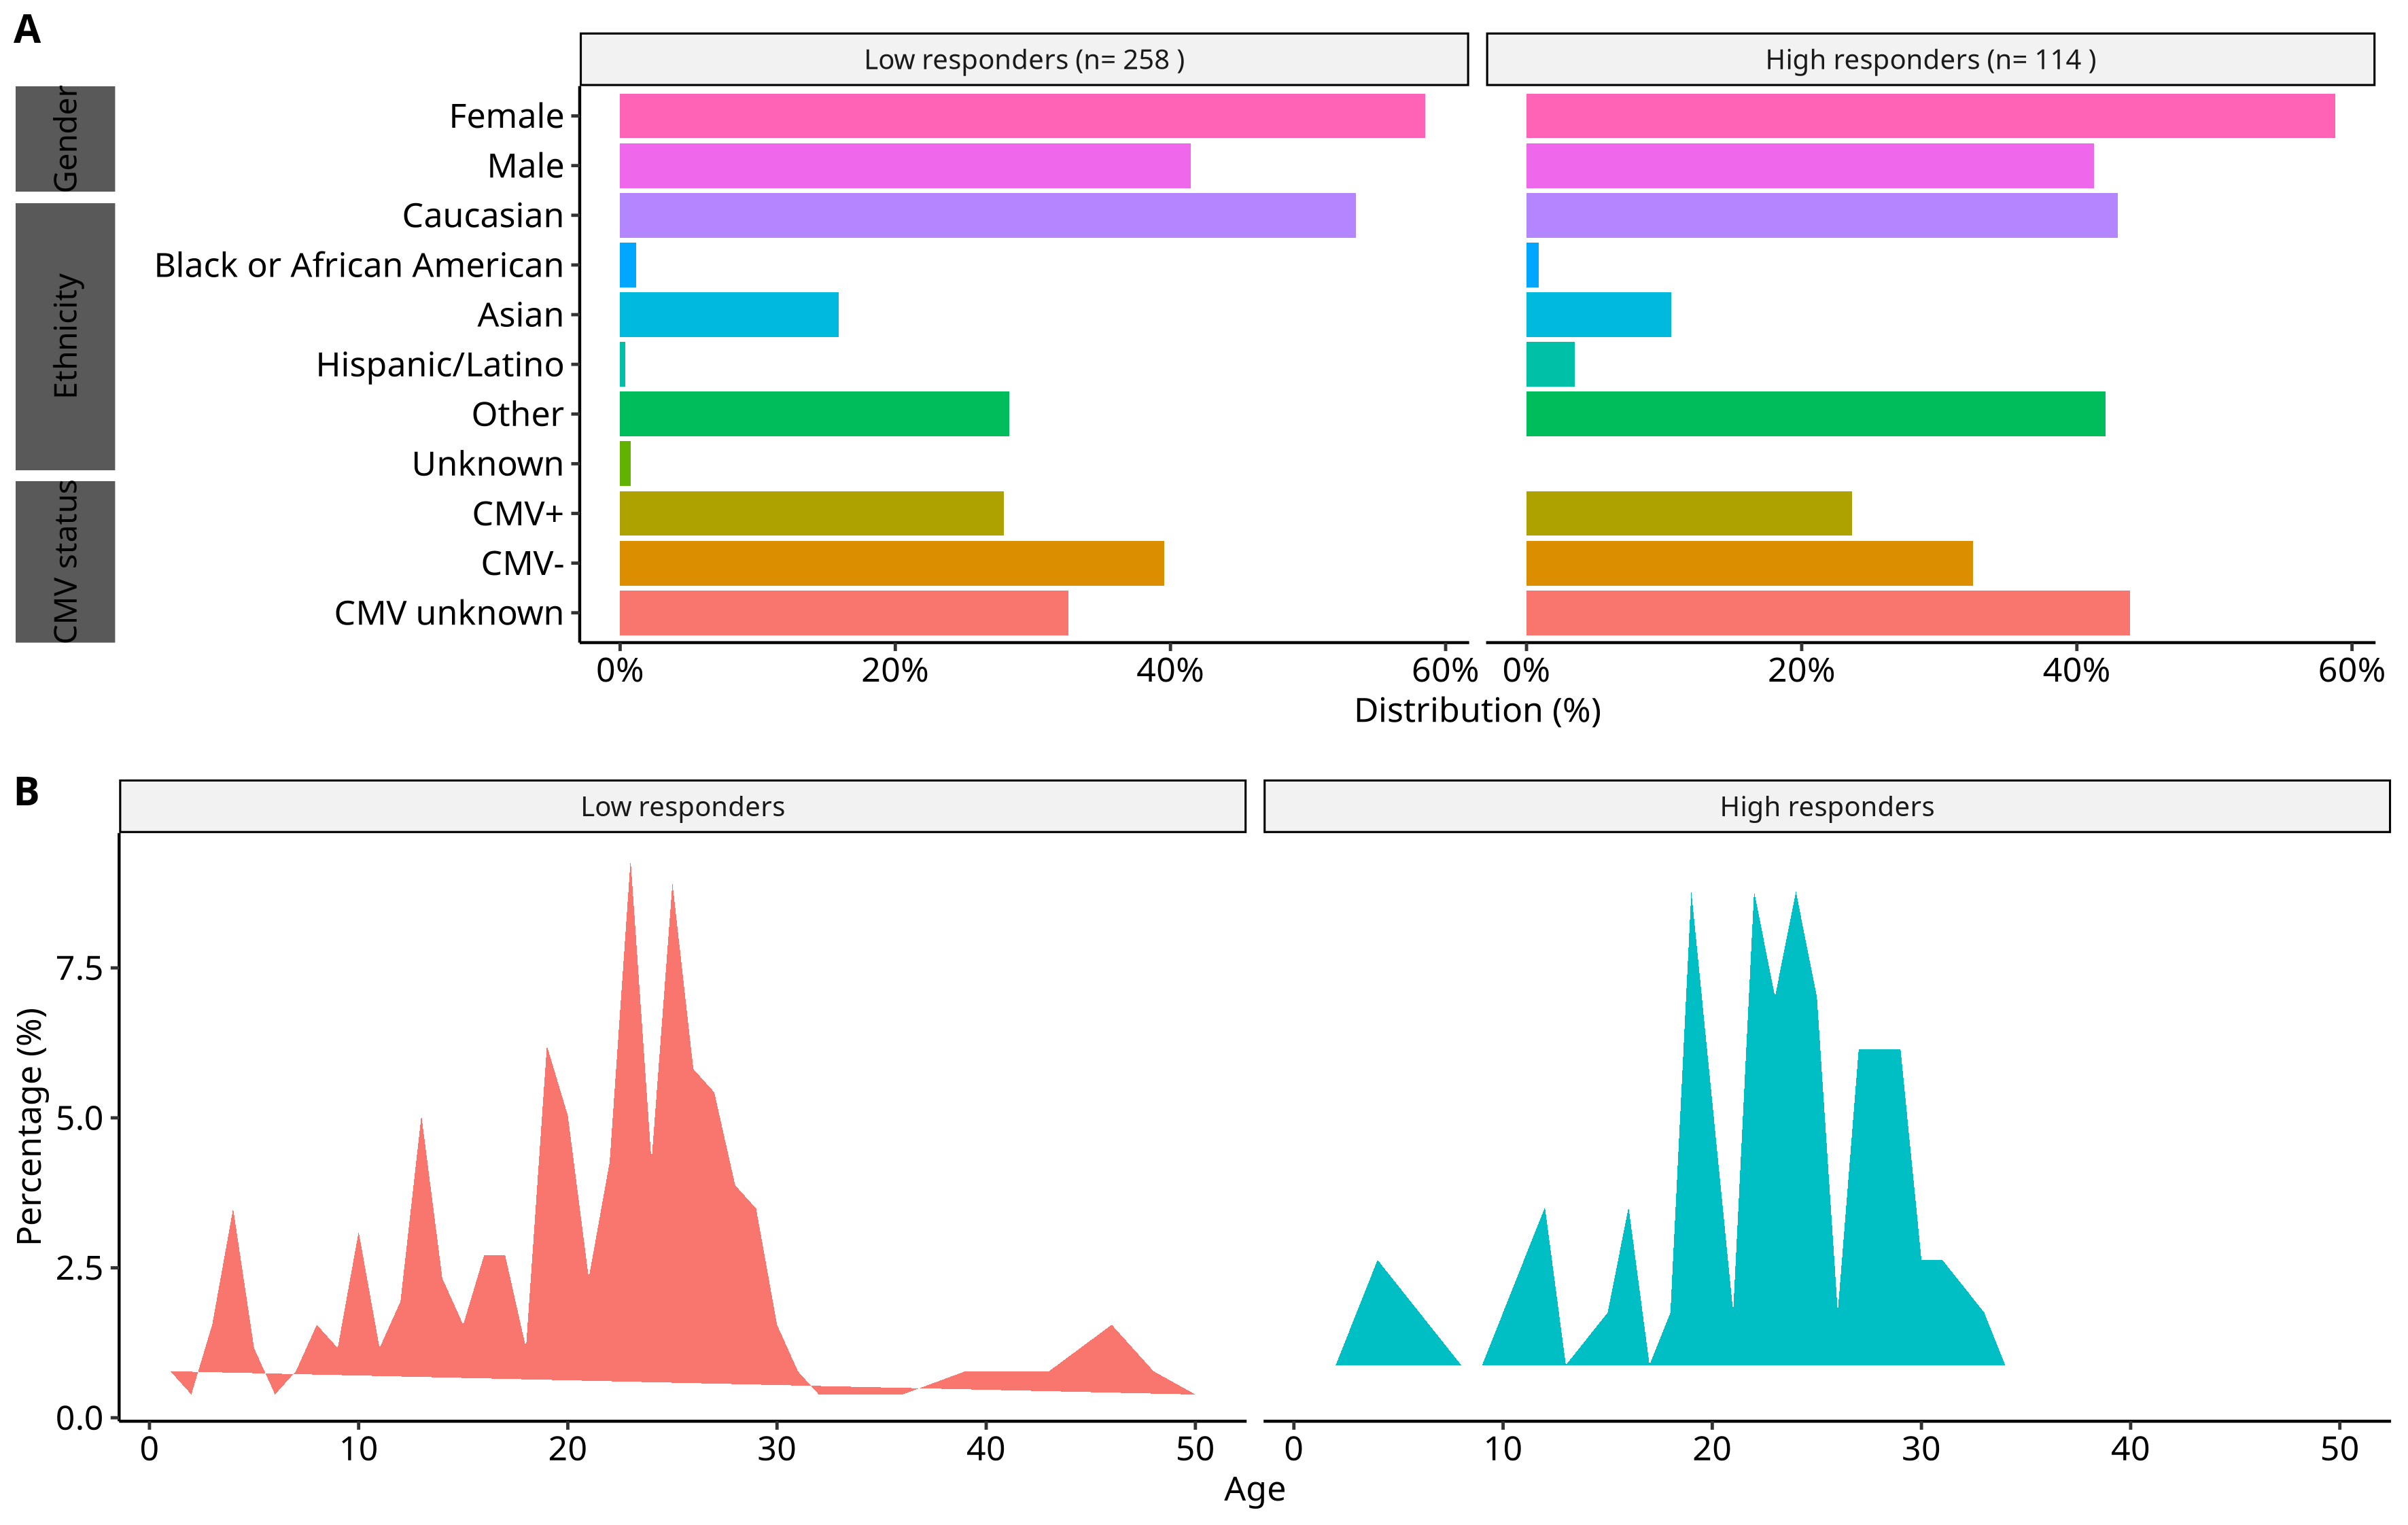
\includegraphics[width=\textwidth]{demographic}
    \caption{\textbf{A.} percentage of donors/rows having some Gender, Ethnicity, or \gls{bu:cmv} status within high and low responder groups.
    \textbf{B.} Age distribution of donors with available response classification.}\label{fig:demoGraph}
\end{figure}



\begin{table}[htpb]
\centering
\begin{tabular}{ll}
\toprule
\textbf{Age (y)} & \\
\midrule
Mean $\pm$ SD & 21.02 $\pm$ 8.66\\
Median (min. to max. range) & 22.5  ( 1 - 50 )\\
\addlinespace
    \textbf{Gender} & \\
\midrule
Male (\%) & 154 ( 41.4 )\\
Female & 218  ( 58.6 )\\
\addlinespace
    \textbf{Ethnicity} & \\
\midrule
Caucasian (\%) & 187 ( 50.3 )\\
African American (Black) (\%) & 4  ( 1.1 )\\
Asian (\%) & 53  ( 14.2 )\\
Hispanic/Latino (\%) & 5  ( 1.3 )\\
Other (\%) & 121  ( 32.5 )\\
Unknown (\%) & 2  ( 0.5 )\\
\bottomrule{}
\end{tabular}
\caption{\textbf{Demographic statistics of donors with known vaccine response classification.}}\label{tbl:demoStats}
\end{table}

The data from the clinical studies consisted of 121 CSV files that were imported into the \flup database.
The data was used to build four tables, three of which were described but we omitted the discussion of technical validation details of the database construction.
The relation between the tables is best visualised using the schema given in \dpaper, it describes the MySql attribute types and columns in the tables \autoref{fig:tablesFluprint} (copied).
The volume of the data is also given in \dpaper, per table the number of rows and columns was reported \autoref{tbl:volumeTables}.

\begin{figure}[htpb]
    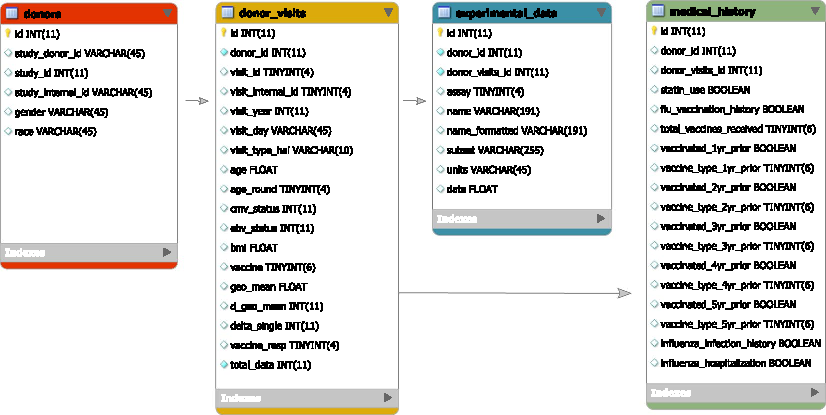
\includegraphics[width=\textwidth]{tablesFluprint}
    \caption{
        \textbf{(taken from original paper)} The \flup database model.
        The diagram shows a schema of the \flup database.
        Core tables, donors (red), donor\_visits (yellow), experimental\_data (blue) and medical\_history (green) are interconnected.
        Tables experimental\_data and medical\_history are connected to the core table donor\_visits.
        The data fields for each table are listed, including the name and the type of the data.
        CHAR and VARCHAR, string data as characters; INT, numeric data as integers; FLOAT, approximate numeric data values; DECIMAL, exact numeric data values; DATETIME, temporal data values; TINYINT, numeric data as integers (range 0–255); BOOLEAN, numeric data with Boolean values (zero/one).
        Maximal number of characters allowed in the data fields is denoted as number in parenthesis.
    }\label{fig:tablesFluprint}
\end{figure}

\begin{table}[htpb]
    \centering
    \begin{tabular}{lll}
        \toprule{}
        \textbf{Table name} & \textbf{Rows} & \textbf{Columns} \\
        \midrule{}
        \textit{donors} &  740 & 6 \\
        \textit{donor\_visits} & 2,937 & 18 \\
        \textit{experimental\_data} & 371,260 & 9 \\
        \textit{Medical history} & 740 & 18 \\
    \bottomrule{}
    \end{tabular}
    \caption{Volume of tables in the Fluprint database.}\label{tbl:volumeTables}
\end{table}

\subsection{Attribute types and values}

Because of the great number of attributes in the database, we discuss them by table starting with the donors table \autoref{fig:tablesFluprint}.

\subsubsection{donors table}

The \textit{id} attribute is simply an enumeration of unique donors, additionally it is used as a key to get attributes from other tables.
The \textit{study\_donor\_id} attribute is an encrypted identification number.
Each donor belongs to the study identified by the \textit{study\_id}, these are the last two digit of the name code (those starting with SLVP0 \(\cdot\cdot\)) in the reference table \autoref{tbl:studiesDesc}, the \textit{study\_internal\_id} is either the digit or a string containing the digit in \textit{study\_id}.
The \textit{gender} and \textit{race} attribute contain the values used in \autoref{fig:demoGraph}, a minor note is that in the original paper "American Indian or Alaska Native" is listed as one of the \textit{race} values but is not used in the database, race attribtue processing is described more in \dpaper.
There are 5 donors whose race is "NULL", which are mapped to unknown \autoref{fig:demoGraph}.

\begin{table}[htpb]
    \begin{tabular}{rlrlll}
\toprule{}
id & study\_donor\_id & study\_id & study\_internal\_id & gender & race\\
\midrule{}
1 & e27ad74ff9a5f2f32d8e852533f054c0 & 30 & 30 & Female & Asian\\
2 & 4a89ac4d3f4dc869e5c8e8cf862cffda & 30 & 30 & Male & Other\\
3 & a2cde6e54dec92422b0427dd49244350 & 30 & 30 & Female & Caucasian\\
4 & 0f7d8d1c13e876017ea465f99d25581f & 30 & 30 & Male & Other\\
5 & 1ed2f6409584b7b4e9720b28d794fe91 & 30 & 30 & Female & Caucasian\\
\addlinespace
6 & a575678405e9615bfb87eccfa031f7fc & 30 & 30 & Male & Other\\
\bottomrule{}
\end{tabular}
    \caption{Head of the donors table.}\label{tbl:donorsHead}
\end{table}

\subsubsection{donor\_visits table}

The donor visits table is the core table of the database, it contains donor attributes at visit times during enrolment in clinical studies in rows that are uniquely identified by an \textit{id} integer.
Each row also includes the \textit{donor\_id} identify the donor that visited by the \textit{id} in the donors table.

The database combines datasets from multiple clinical studies spanning multiple years.
Within clinical studies the data is often incomplete due to factors that change between influenza seasons, such as changes in the number of features measured in an assay data collected.
As a result, the \flup database is incomplete and contains heterogeneous data quality \autoref{tbl:visitsDesc}.
More, every attribute in the core table has missing values, which complicates selection of data for further analysis.
In summary, the number of visits is inconsistent per season per donor, all columns are incomplete, and classification is sometimes based on single visits or inconsistent with available data \autoref{tbl:visit166} \autoref{tbl:visitsDesc}.

\begin{table}[htpb]
\addtolength{\leftskip} {-2cm} % increase (absolute) value if needed
\addtolength{\rightskip} {-2cm} % increase (absolute) value if needed
\begin{tabular}{lrrrrrrrrr}
\toprule{}
stat & age & cmv\_status & ebv\_status & bmi & vaccine & geo\_mean & d\_geo\_mean & vaccine\_resp & total\_data\\
\midrule{}
n & 2937.0 & 1081.0 & 548.0 & 516.0 & 2794.0 & 984.0 & 1260.0 & 1206.0 & 2937.0\\
na & 0.0 & 1856.0 & 2389.0 & 2421.0 & 143.0 & 1953.0 & 1677.0 & 1731.0 & 0.0\\
mean & 47.3 & 0.4 & 0.8 & 24.8 & 3.7 & 87.6 & 8.9 & 0.3 & 126.4\\
sd & 27.0 & 0.5 & 0.4 & 5.6 & 1.0 & 101.7 & 30.9 & 0.4 & 368.4\\
se\_mean & 0.5 & 0.0 & 0.0 & 0.2 & 0.0 & 3.2 & 0.9 & 0.0 & 6.8\\
\addlinespace
IQR & 50.2 & 1.0 & 0.0 & 6.7 & 0.0 & 105.4 & 4.0 & 1.0 & 19.0\\
skewness & 0.2 & 0.3 & -1.4 & 1.0 & -1.7 & 3.6 & 9.9 & 1.1 & 7.1\\
kurtosis & -1.5 & -1.9 & -0.1 & 2.1 & 3.0 & 26.6 & 114.9 & -0.9 & 49.7\\
\bottomrule{}
\end{tabular}
\caption{
    Descriptive stats of relevant numeric or binary factor columns in the donor visits table.
    For geo\_mean 0 is considered as missing data.}\label{tbl:visitsDesc}
\end{table}

Per donor all visits are enumerated in chronological order by \textit{visit\_id} \autoref{tbl:visit166}.
Further visit info includes: \textit{visit\_internal\_id} which is a number that indicates the visit order within an influenza season but this differs per clinical study (e.g. some use 1-2-3, orther use 0-7-28), the \textit{vist\_year} is the influenza season of the visit, the \textit{visit\_day} is the number of days relative to the date of vaccination,  \textit{age} and \textit{age\_round} indicate the donor's age at time of the visit, and \textit{bmi} gives the donor bmi at visit time, and lastly \textit{visit\_type\_hai} is the intent of the visit which is either "pre", "post", "other", or "single".

Depending on clinical study, during the "pre" visit a virological assay is performed to determine the \gls{bu:cmv} and \gls{bu:ebv} status of the donor, which are indicated by the binary variables \textit{cmv\_status} and \textit{ebv\_status}.

In most clinical studies, vaccine response was measured using the \gls{bu:hai} assay.
The procedure measures the influenza antibody titers before vaccination during the \textit{visit\_type\_hai} "pre" visit of a participant, and 28 days after vaccination during a "post" visit.
The \acrshort{gmt} at each visit is calculated, and a fold change in \acrshort{gmt} is calculated as the ratio of the \acrshort{gmt} at day 28 (post) and during the first visit (pre).
These values are called \textit{geo\_mean} and \textit{d\_geo\_mean}, respectively.
Lastly, there is one more \gls{bu:hai} related data attribute which is the \textit{d\_single}, this is reported as the antibody \gls{bu:titer} fold-change per strain of virus used in the vaccine.
It is unclear how this value is aggregated over different influenza strains in a \gls{bu:tiv} and is left out of further analysis.
Based on these \gls{bu:hai} related attributes a donor is classified as high or low responder, the seasonal vaccine response classifications are given by the \textit{vaccine\_resp} attribute.

The type of vaccine used in a study is indicated by the \textit{vaccine} attribute, the meaning of the vaccine id is reported in the appendix \autoref{tbl:remapVaccine}.
The type of experimental assays performed to measure the immunological profile of the donor during the "pre" visit are described later in the section of the experimental data table.
All assays are listed in \dpaper and are summarised here \autoref{tbl:assays}.
This information is relevant to \textit{total\_data} attribute of the donor visits table which indicates the number of measurements made during a visit.

\begin{table}[htpb]
\addtolength{\leftskip} {-2cm} % increase (absolute) value if needed
\addtolength{\rightskip} {-2cm} % increase (absolute) value if needed
\begin{tabular}{rrrlrrrlrrrrr}
\toprule{}
visit\_id & year & day & type & age & cmv & ebv & bmi & vaccine & geo\_mean & d\_geo\_mean & response & assay\_data\_rows\\
\midrule{}
1 & 2011 & 0 & pre & 20 & 1 & 1 & 30.31 & 4 & 25.20 & 6 & 0 & 343\\
2 & 2011 & 7 & other & 20 & 1 & 1 & NULL & 4 & 0.00 & 6 & 0 & 51\\
3 & 2011 & 28 & post & 20 & 1 & 1 & NULL & 4 & 160.00 & 6 & 0 & 51\\
\addlinespace
4 & 2012 & 0 & pre & 21 & 1 & 1 & 30.31 & 4 & 9.28 & 4 & 0 & 292\\
\addlinespace
6 & 2013 & 0 & pre & 22 & 1 & 1 & 30.31 & 4 & 15.91 & 2 & 0 & 2877\\
7 & 2013 & 7 & other & 22 & 1 & 1 & NULL & 4 & 0.00 & 2 & 0 & 63\\
8 & 2013 & 28 & post & 22 & 1 & 1 & NULL & 4 & 26.75 & 2 & 0 & 82\\
\bottomrule{}
\end{tabular}
\caption{
    Visit data of donor 166 from study SLVP021 \autoref{tbl:studiesDesc}.
    Note that the number of visits and volume of data collected at visit varies per season.
    Further, the classification is inconsistent with \gls{bu:seropc} criteria in 2011.}\label{tbl:visit166}
\end{table}

The most important data related to the visits of donor 166 is shown in Table \ref{tbl:visit166}.
As described above, the vaccine response classification is determined per season based on the \acrshort{gmt} in the "pre" and "post" visits.
However, since the \gls{bu:hai} assay requires a "pre" visit and a "post" visit 28 days later to measure the difference in GMT, a classification is inconsistent when there is only one visit record in a season \autoref{tbl:visit166}.

\begin{figure}[htpb]
    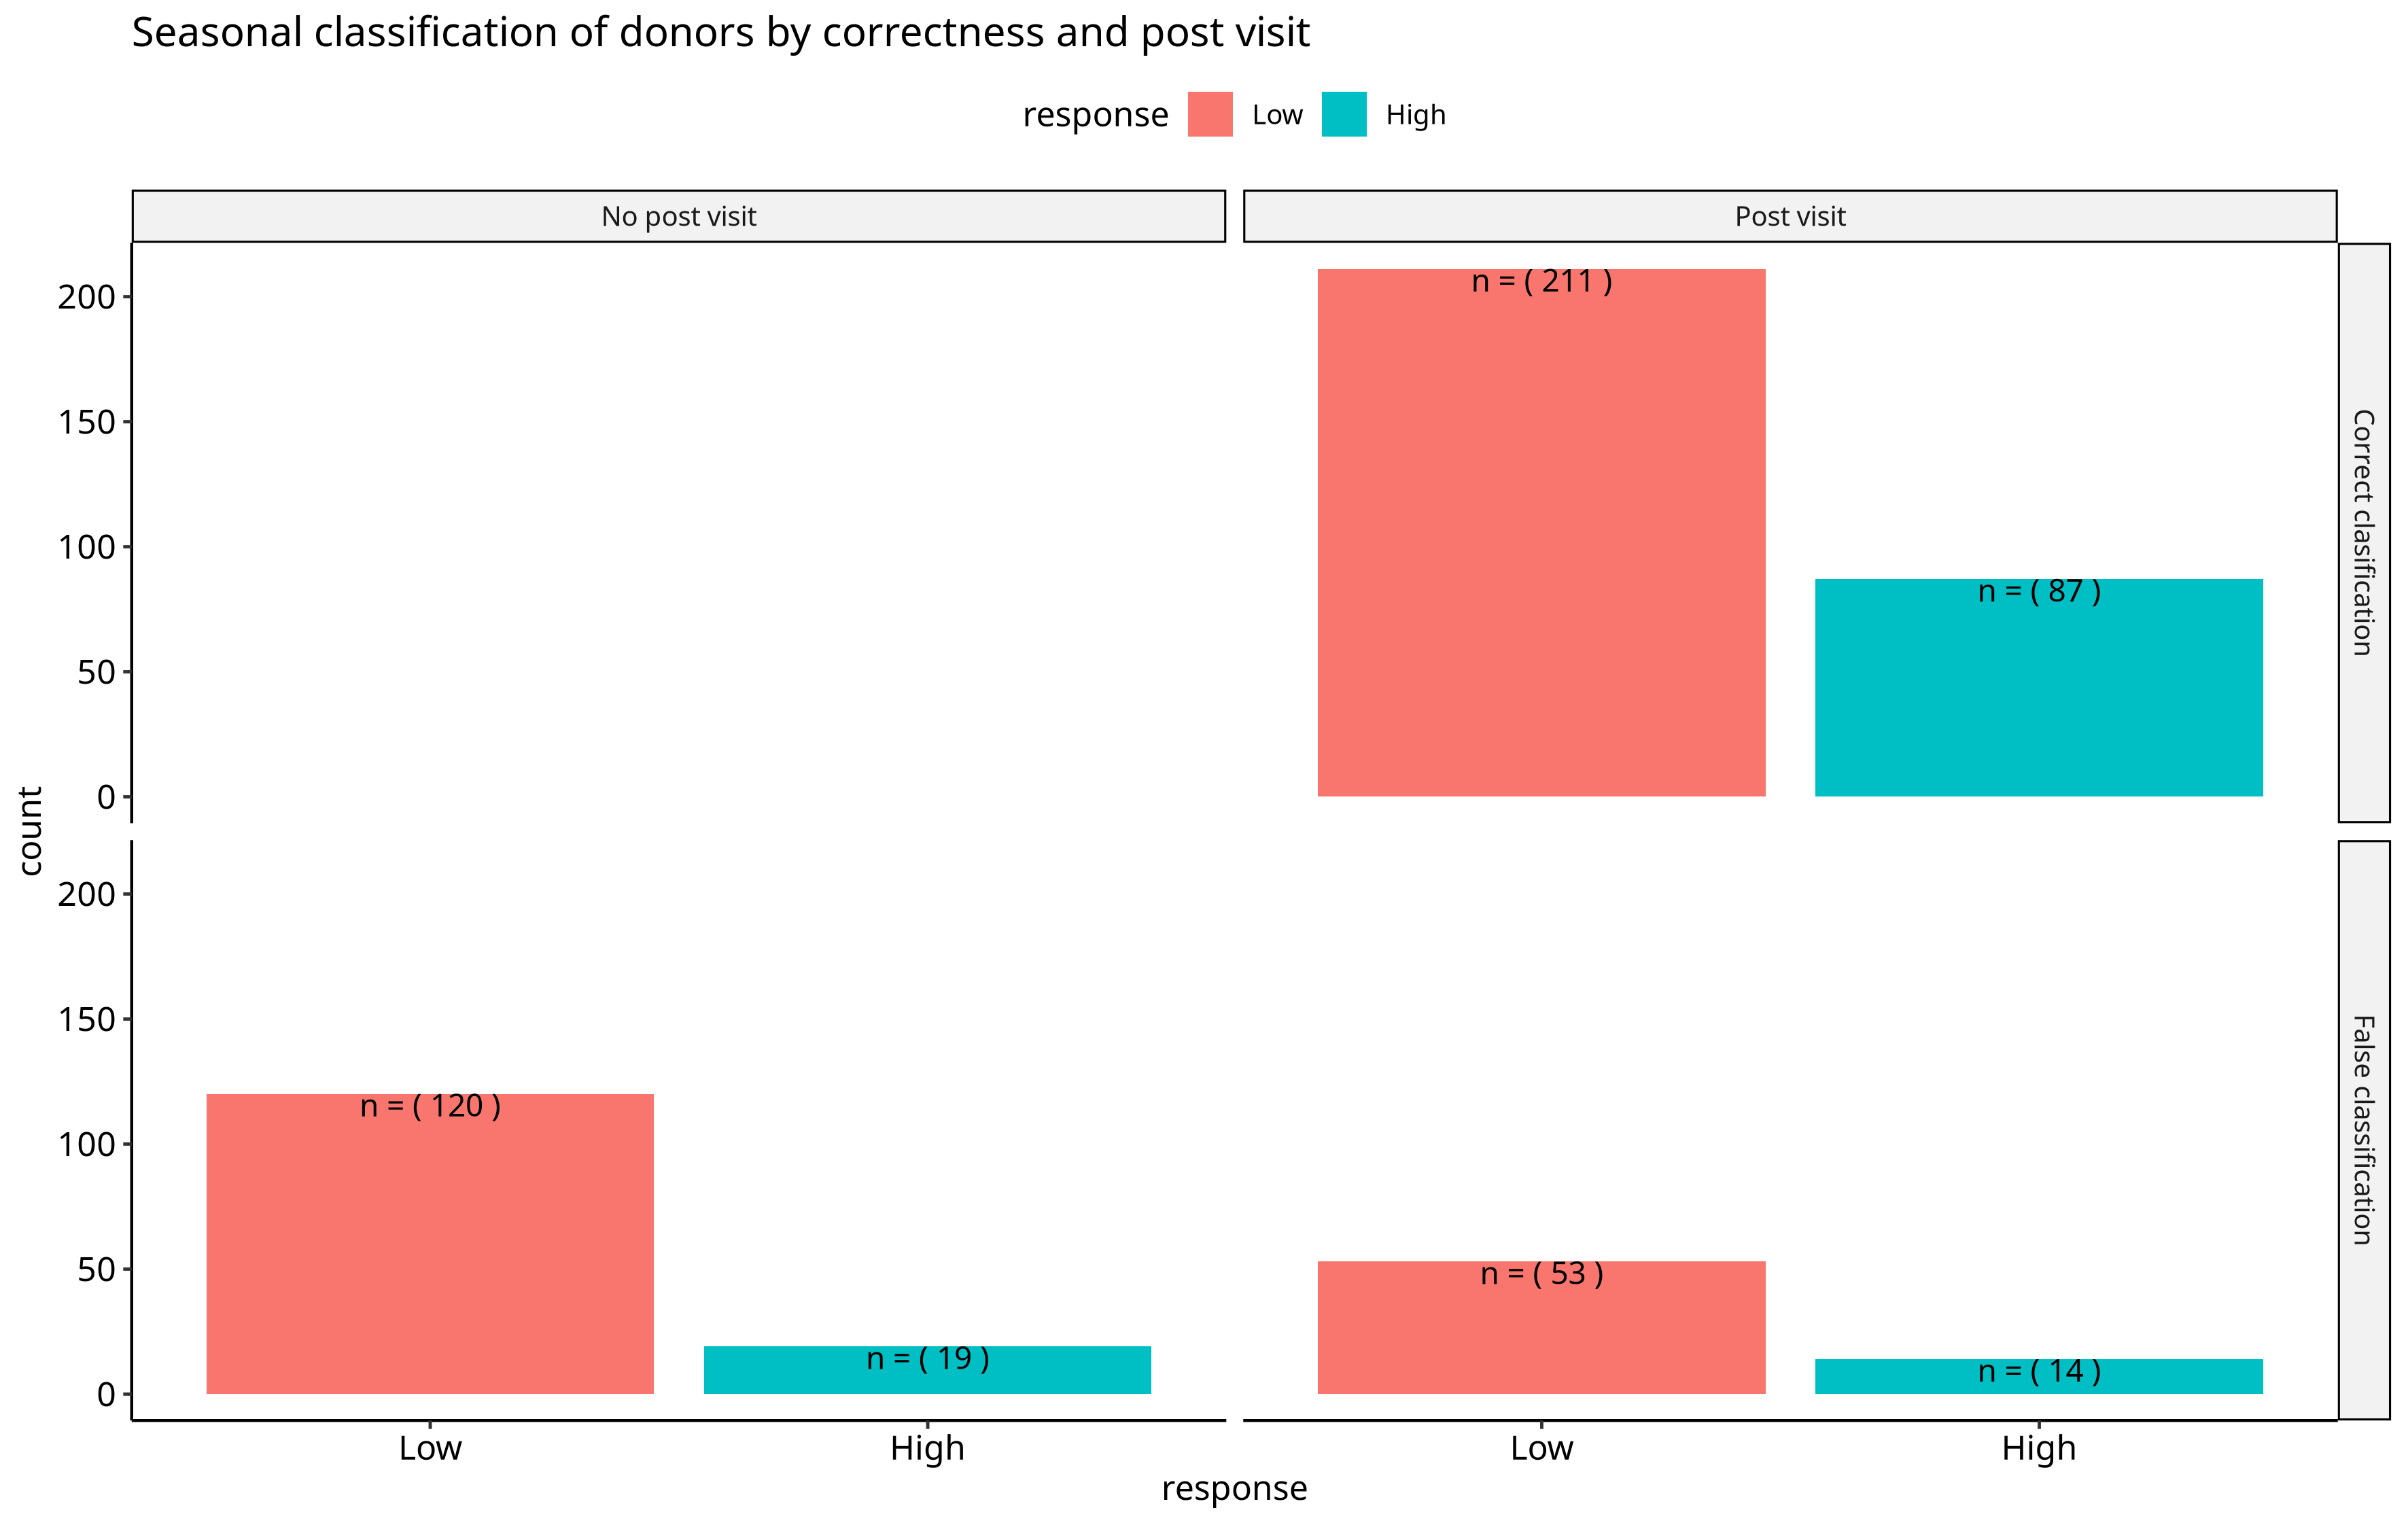
\includegraphics[width=\textwidth]{season_classification}
    \caption{
        \textbf{Classifications inconsistent with \gls{bu:seropc} criteria using given data.}
        The classifications given in influenza seasons with only a visit with \textit{visit\_type\_hai} value of "single" or "other", or did not have "pre" and "post" visits were considered inconsistent with the \gls{bu:hai} procedure.
        Additionally, those that did not meet the \gls{bu:seropc} criteria given the \acrshort{gmt} data were considered inconsistent.
    }\label{fig:classInconsistent}
\end{figure}

Furthermore, the example of donor 166 contains another type of inconsistency in the classification, in 2011 the GMT \textit{geo\_mean} increases from 25.20 to 160.00, and the \textit{d\_geo\_mean} is 6, but in this season the donor is classified as a low responder, even though \gls{bu:seropc} criteria are met \autoref{tbl:visit166}.
Because of these apparent inconsistencies the seasonal classification of donors was evaluated using available \acrshort{gmt} data and the \gls{bu:seropc} criteria \ref{fig:classInconsistent}, records of incorrectly labelled donors are also saved as a spreadsheet.
Given the information in the database classification is inconsistent in a large number of cases.
However, the most likely explanation is that antibody \gls{bu:titer} for one specific strain of virus in the vaccine did not meet the \gls{bu:seropc} criteria.
Therefore, in this work it was considered as inconsistent because classification required data not given in the database.
Nevertheless, the classification is not necessarily incorrect and the classification data was used in this work without any modifications.

\subsubsection{experimental\_data table}

\begin{table}[htpb]
    \begin{tabularx}{\textwidth}{Xp{0.5\textwidth}X}
\toprule{}
        \textbf{Name} & \textbf{Description} & \textbf{id} (\textit{experimental\_data.assay})\\
\midrule{}
        (Multiplex) cytokine assays & Multiplex ELISA using Luminex polysterene
        bead or magnetic bead kits. Measures serum cytokine/hormone level in
        z.log2 units using fluorescent antibodies. & 3, 6, 15, 16\\
        \addlinespace
        Flow and mass cytometry assays & uses labeled antibodies to detect antigens on
        a cell surface to identify a subset of a cell population, units are in
        percentage of parent population. & 4, 9, 13, 17 \\
        \addlinespace
        Phosphorylation cytometry assays & Uses antibodies to measure
        phosphorylation of specific proteins stimulated by an immune system event
        belonging to cell population subsets. Units are a fold change between
        stimulated and un-stimulated cells, for mass cytometry arcsin readout difference,
        fold-change of 90th percentile readout values otherwise.  & 7, 10 (mass cytometry) (flow cytometry)\\
        \addlinespace
        complete blood count (CBCD) & Different cells are counted using flow
        cytometry Units are usually in Count/$\mu$L & 11 \\
        \addlinespace
        meso scale discovery assays (MSD) & A setup where serum cytokines or hormones
        are captured with antibodies, and then detected by using a detection
        antibody. Units are arbitrary intensity & 2, 12, 14 \\
\bottomrule{}
\end{tabularx}
    \caption{
        Table containing the types of data collected at donor visits.
        It describes the assay type in the name and description columns.
        The id column refers to the different specific assays belonging to a data type with the id used in the database.
        The mapping from id to assay can be found in the appendix \autoref{tbl:remapAssays}.
    }\label{tbl:assays}
\end{table}


\fpfig{exp_data_numbers}{.7}
{
    Description of data volume collected in different years and studies, by data type or experiment id and stratified by classification.
}
{
    \textbf{A.} the aggregated number of data points/features measured per season and by classification.
    Data is shown per experiment id used in the \flup database, indicated with color.
    \textbf{B.} Same as (\textbf{A}), but grouping experiments per data type instead of experiment id, the same as in (\textbf{C}).
    \textbf{C.} Seasonal data points per data type by study instead of classification.
}
{fig:featureNumbers}

As reported in \dpaper different assays performed in clinical studies are remapped to and \textit{id} number, but the values in the database do not correspond to the reported remaps \autoref{tbl:remapVaccine}.
The actual data type, units, and assay id contained in the database were described in this work \autoref{tbl:assays}.

In total there are 14 different experimental assays used across clinical studies, not counting the virological and \gls{bu:hai} assays \autoref{tbl:assays}.
Further, the virological assays determining the \gls{bu:cmv} and \gls{bu:ebv} status are not used in this work, since it is available only in a small subset of the collected data.
Those 14 assays have been aggregated in this work to 5 different data types/experiment types \autoref{tbl:assays}, in short:

\begin{itemize}
    \item the multiplex cytokine assays measure levels of molecules such as \gls{bu:cytokine}s and other signaling molecules in human serum/blood,
    \item flow and mass cell cytometry measure the phenotype of specific immune related cells,
    \item phosphorylation flow and mass cytometry measures signaling pathway activation after an induced \gls{bu:cytokine} stimulation or the absence thereof,
    \item the complete blood count (CBCD) measures the concentration of cells in the serum/blood,
    \item and meso scale discovery (MSD) measures hormones or cytokines from human serum/blood.
\end{itemize}

\begin{figure}[htpb]
    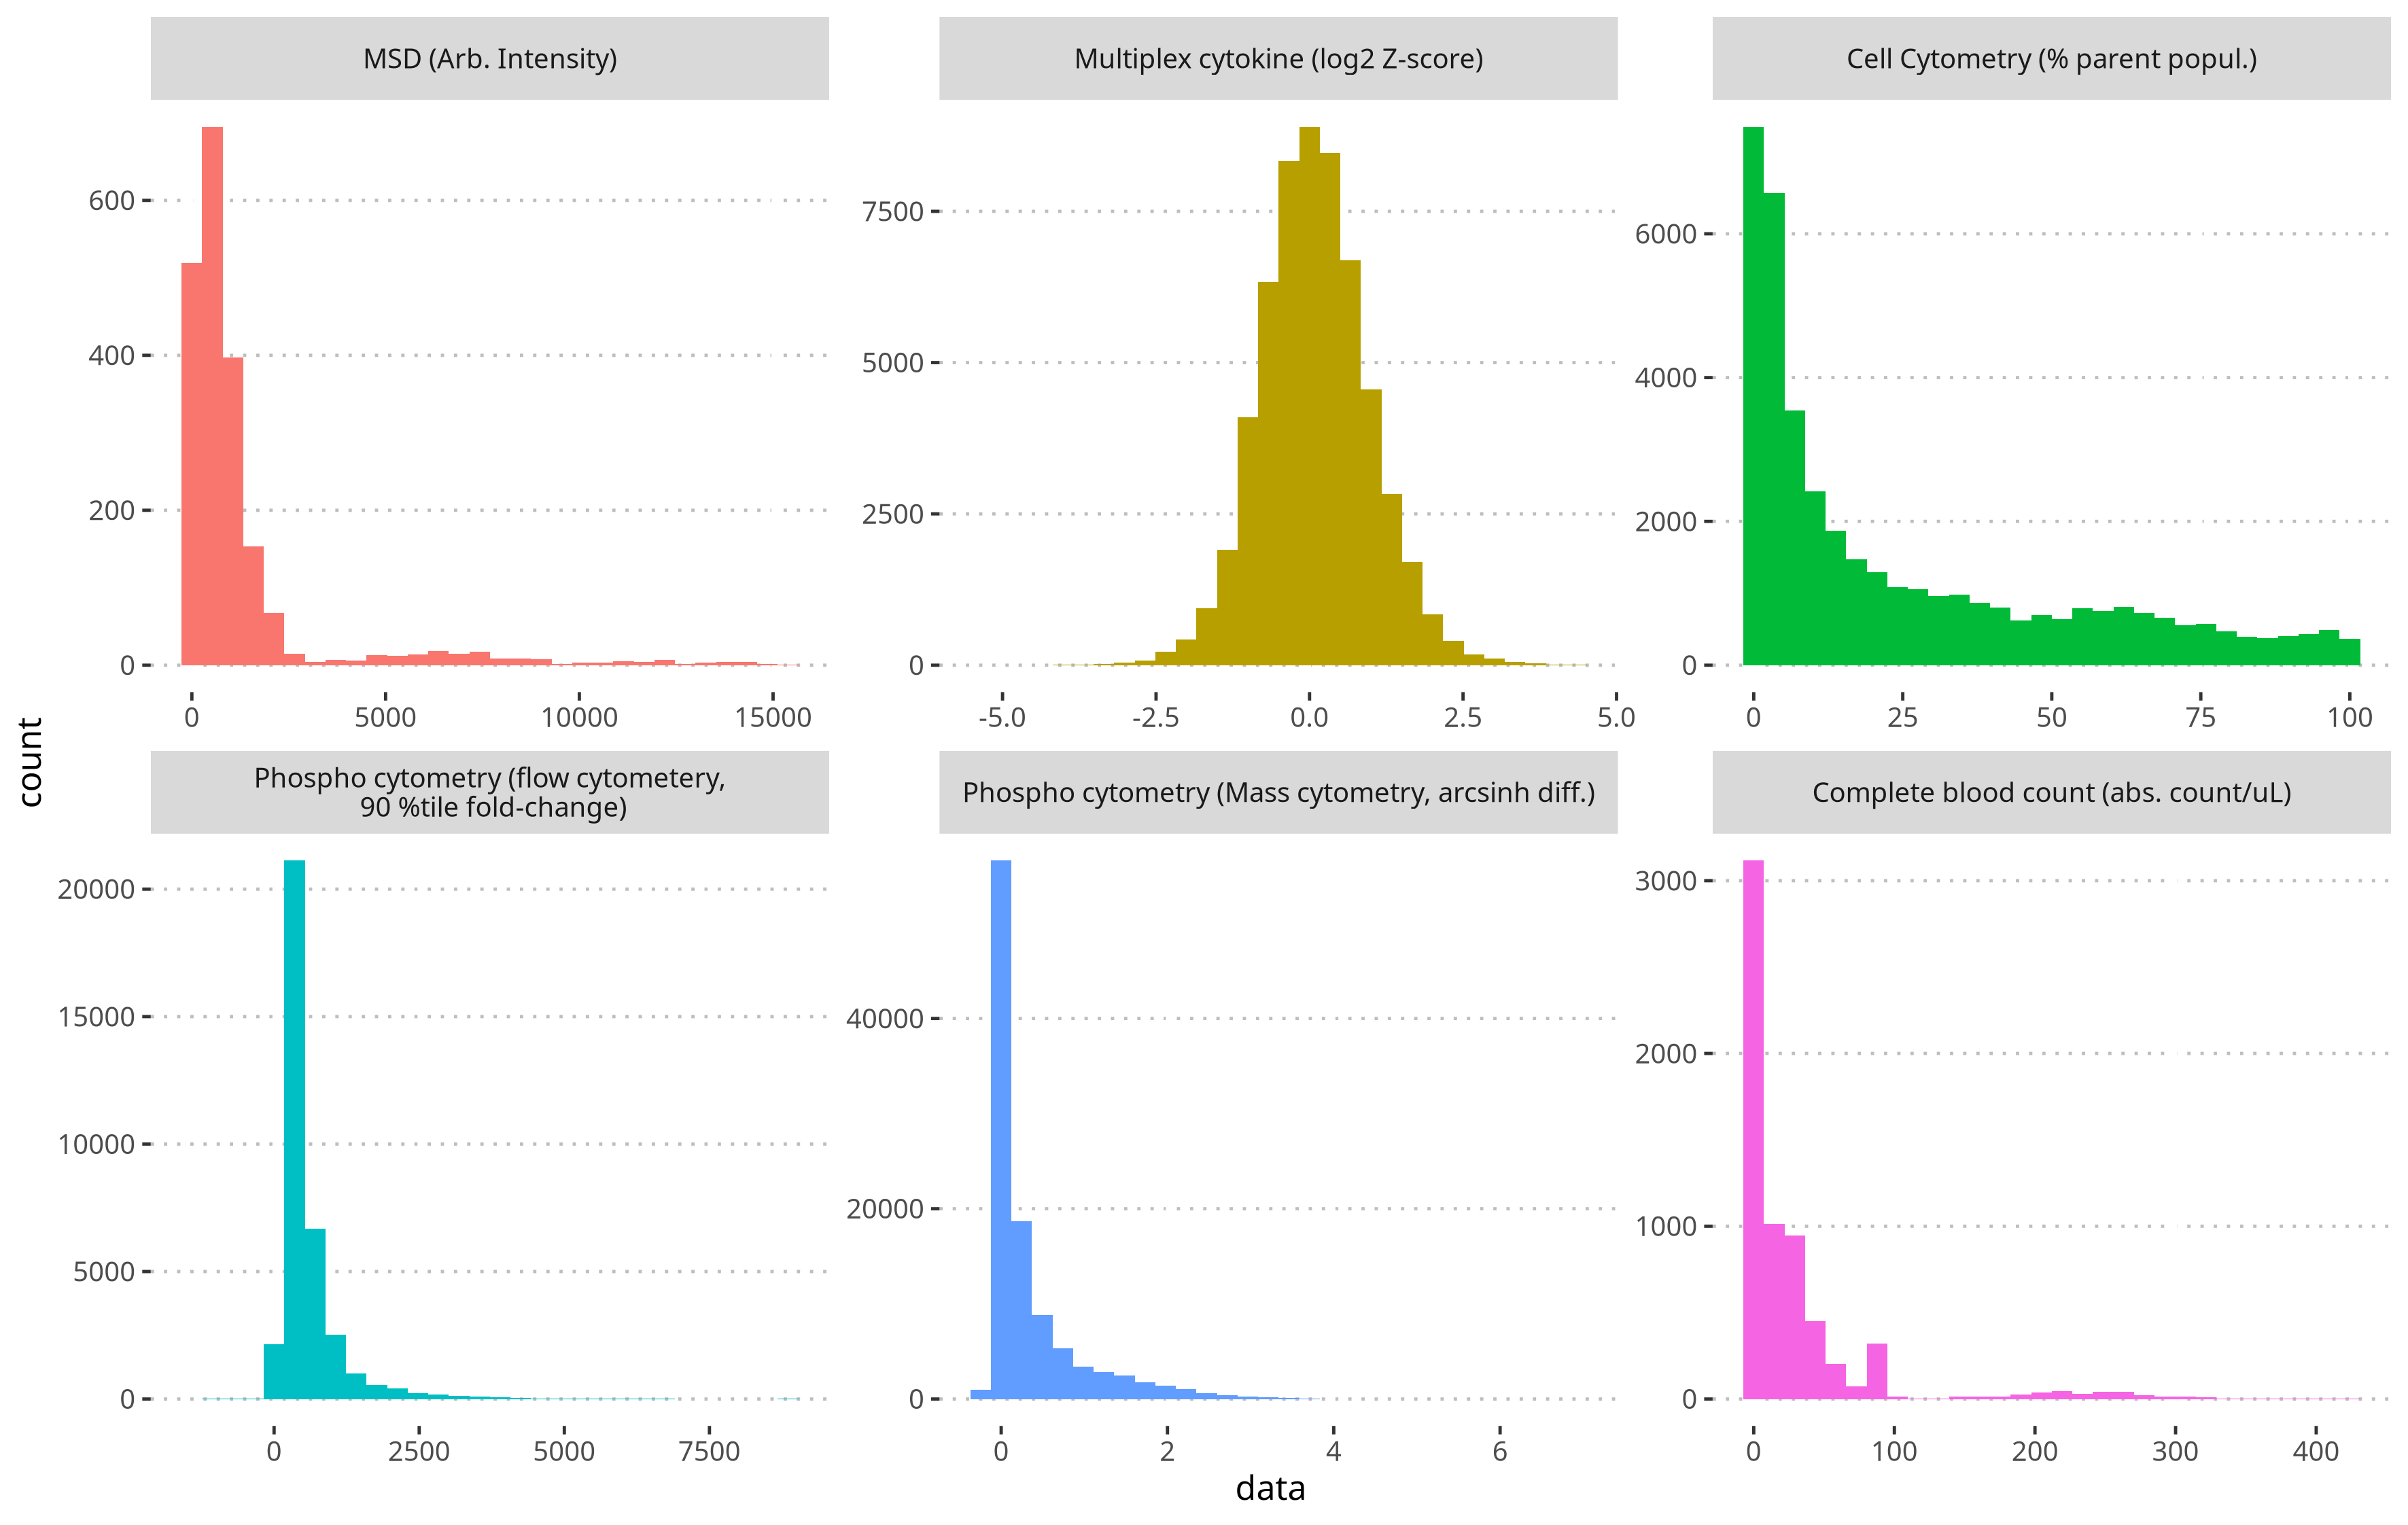
\includegraphics[width=\textwidth]{assay_value_distributions}
    \caption{noise in 90th \%tile}\label{fig:assayDistr}
\end{figure}

The experimental data table contains all features recorded per donor visit.
The number of features collected for each visit is large and varies greatly (mean at 126 , \(\pm \)368 SD) \autoref{tbl:visitsDesc}, and in total there are 3285 different features measured across all clinical studies.
However, not every assay is done in every clinical study  and over the years the data generated by assays has changed, so a table with all features as columns and all donors as rows would be extremely sparse \autoref{fig:featureNumbers}.
Describing the 3285 different features in this sparse table would be impossible, but assay value distributions across studies are shown to follow normal or power distributions \autoref{fig:assayDistr}.

\begin{figure}[htpb]
    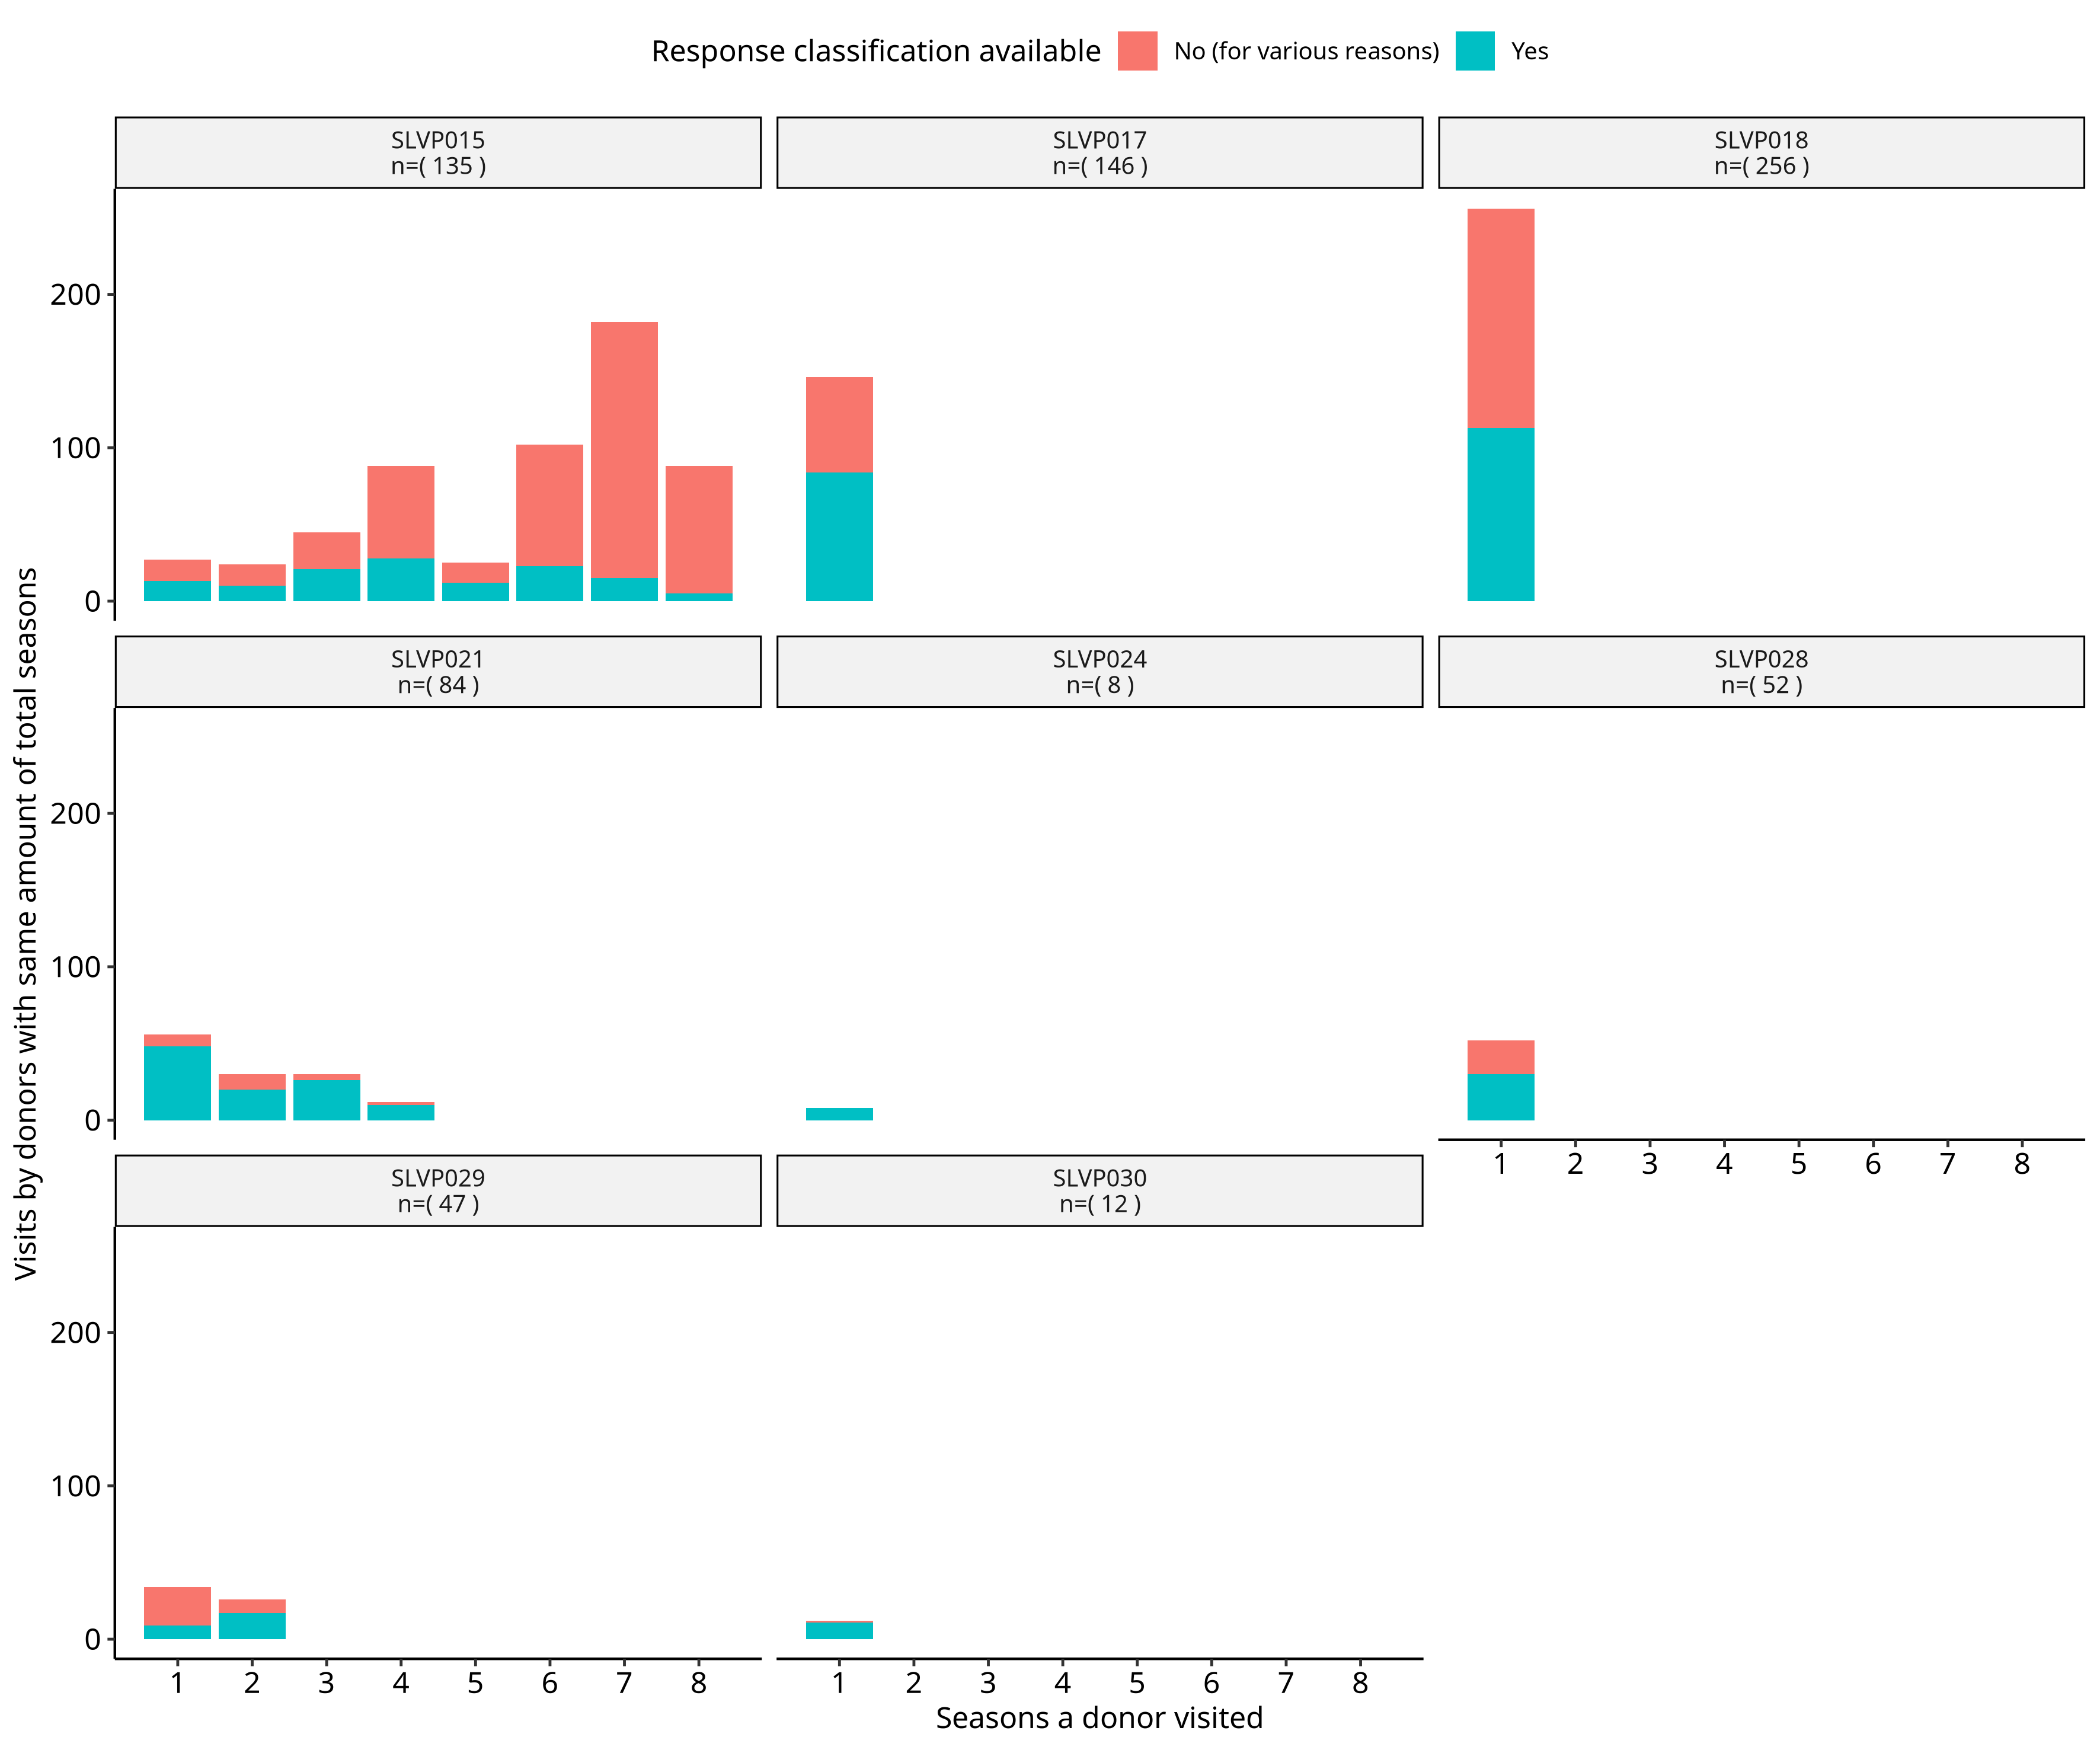
\includegraphics[width=\textwidth]{repeat_visits_per_study}
    \caption{the number of donors that visited per number of influenza seasons
    they visited (years), per study. The color indicates the number of visits for which a
    classification was available, counted within the groups of donors that
    visited the same amount of times.}\label{fig:repeatVisits}
\end{figure}

In addition to the sparseness of data, what further complicated selecting relevant data is repeat visits of donors, and missing visits.
The problem of repeat visits over a span of multiple influenza seasons is the change in the data type collected per season, and that repeat visits are only a small portion of the database.
Furthermore, the potential for studying the effect of repeat vaccination on high versus low vaccine response classification is limited, since the classification in the longitudal study (SLVP015) containing repeat visit data is not available in a majority of data points \autoref{fig:repeatVisits}.
As a result, exploring what effect repeat vaccination has on vaccine response was done in this work using the small subset of donors where a classification was available in two influenza seasons.

\subsection{Data quality}

The database has issues that are inherent to combining multiple studies.
Firstly, the vaccine response classification was inconsistent with the given data in some cases \autoref{fig:classInconsistent}.
Secondly, the classification was often missing completely because no \gls{bu:hai} assay data was available.
Thirdly, the classification was set to a null value by the database authors because possibly the antibody titer for a single strain of virus in the vaccine was too low (this data is not in the database) \autoref{fig:repeatVisits}.
Lastly, the data is highly sparse when considering data collected on donors in different studies or in different influenza seasons.

The value of the database in terms of knowledge is the great amount of assay data that was collected in different studies across years and was preprocessed.
But this information is hard to access since all studies do not use different assays \autoref{fig:featureNumbers}, resulting in high sparsity data.
Further, the sample size that can be used for further classification studies is limited, since the high versus low vaccine response is only available for a minority of the data points.

\section{Data preparation}

\subsection{Data selection}

The data used in this work was based on the data used in \spaper \autoref{lst:QueryTemplate}.
Using this query template generates a subset of \flup comprised data from 5 clinical studies using the same vaccine type \autorefsub{tbl:remapVaccine}{Vaccine id 4}, most importantly the longitudinal study SLVP015 \autoref{tbl:studiesDesc}.
Presumably the authors of \spaper included only the first visit of donors because the classification is the most complete in this dataset \autoref{fig:dataRepeatvisits}.
In this work we firstly use this query to generate initial first visit datasets.
Secondly, to explore repeat vaccination, we select a subset of this data that includes only donors with a repeat visit in a second influenza season.

\begin{figure}[htpb]
    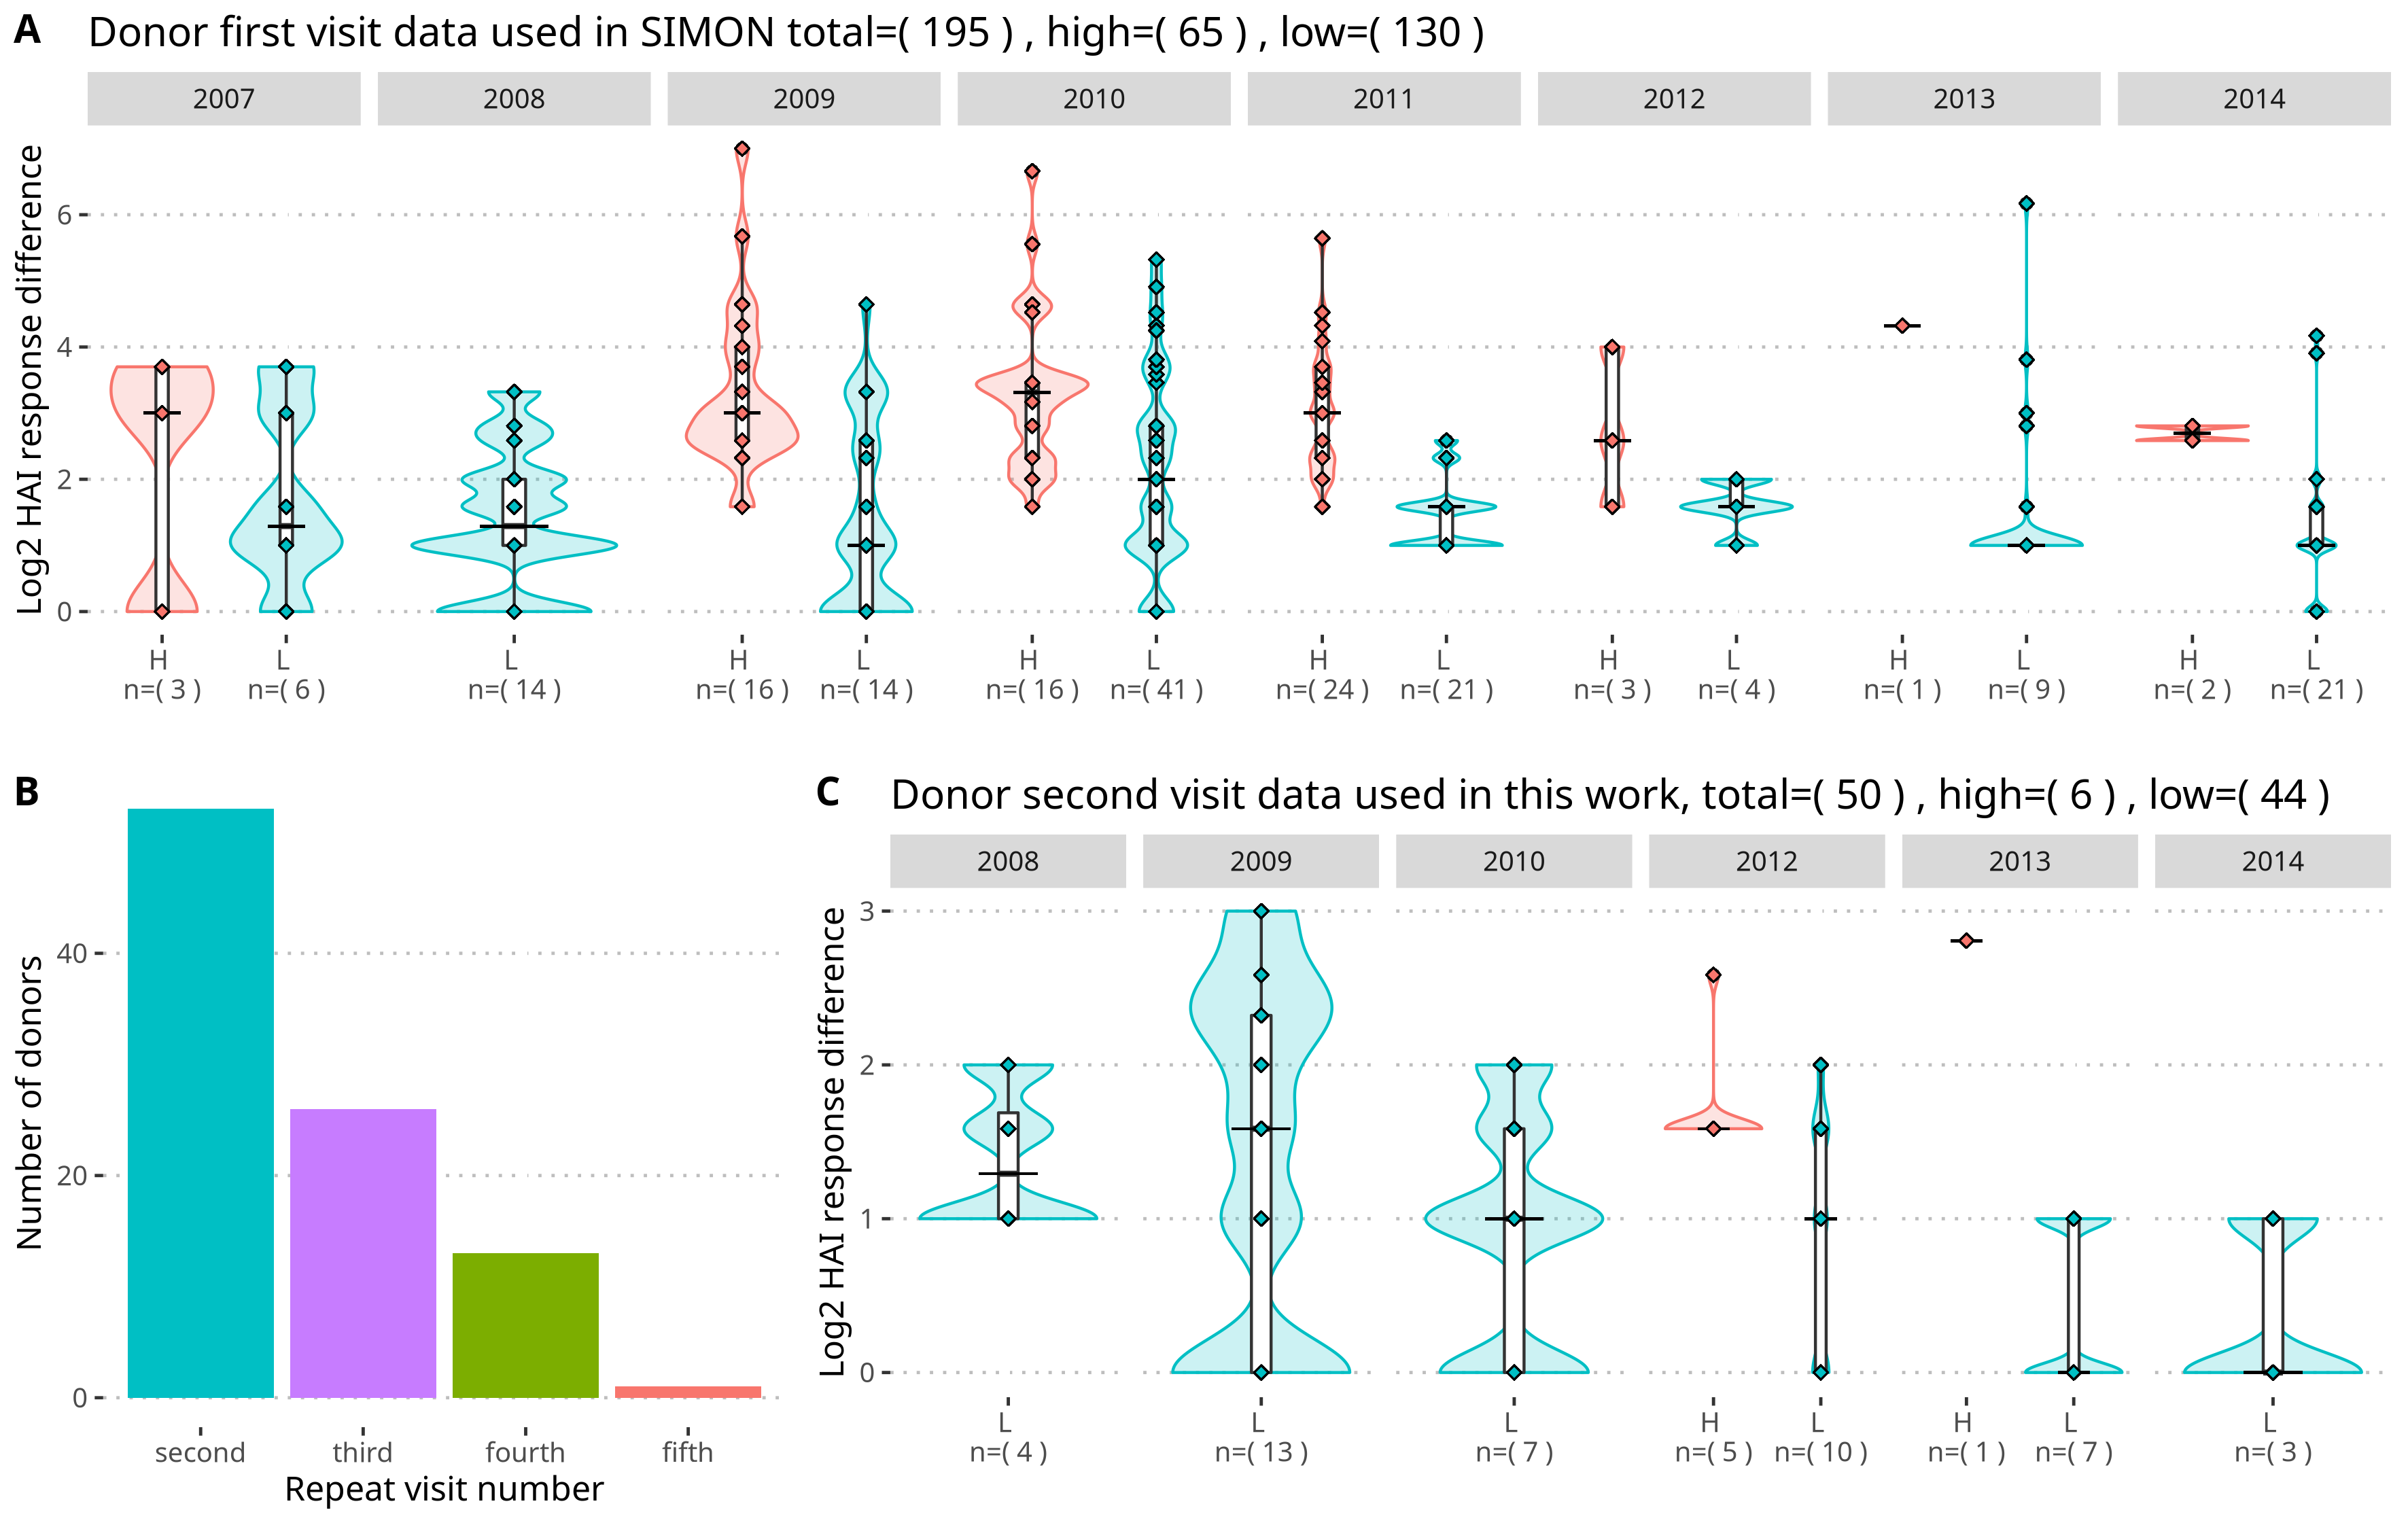
\includegraphics[width=\textwidth]{data_selection}
    \caption{caption}\label{fig:dataRepeatvisits}
\end{figure}

The initial query generated a long table for in total 3285 different features recorded at the first visit of 195 donors in different studies and years (referred to as \firstvis).
An observable pattern in this data is that low responding donors are overrepresented and that the classification is mostly consistent with the \gls{bu:seropc} criteria as seen by the log2 \acrshort{gmt} change feature \autorefsub{fig:repeatVisits}{A}.
Unfortunately, the number of donors in the \firstvis that returned in other influenza seasons decreases quickly, limiting possibilities of comparing models built on \firstvis and subsequent visit data \autorefsub{fig:repeatVisits}{B}.
The selected \secondvis lacks the high response class (except for 6 donors) precluding training any models, therefore we only used the \secondvis to explore the knowledge gained by models trained on the \firstvis \autorefsub{fig:repeatVisits}{C}.

\begin{minipage}{\linewidth}
\begin{lstlisting}[caption=Applying the mulset algorithm and preparing the data, label={lst:mulsetStep}]
generate intersection datasets suitable for analysis
for {each donor in data} do:
    Calculate intersection between donor and all other donors using mulset algorithm
    Skip sets that have less than 5 features and less than 15 donors in common
end for;

for {each set in generated datasets} do:
    Partition data in training (75\%) and test (25\%) split
    Skip sets that have less than 10 donors in the test set
end for;

for {each set in prepared datasets} do:
    calculate number of donors that visited a second influenza season
    skip dataset if it is not in the top3 of datasets containing the highest number of second visitors
end for;
\end{lstlisting}
\end{minipage}

The \firstvis used for modeling and feature selection had a total of 640575 cells of which 596736 values were missing (sparsity of 93\%).
In \spaper missing values in this data is not imputed because there is not enough prior knowledge.
And, since every donor had a missing feature, dropping all rows/donors was not an option either.
A solution used in \spaper was generating complete tables comprising small subsets of donors that had all features in common using the mulset algorithm \autoref{lst:mulsetStep} \autoref{fig:mulsetAlg}.

In this work the procedure in \spaper was replicated and extended to generate usable datasets for feature selection \autoref{lst:mulsetStep}.
First, there were duplicate measurements of features in the \firstvis, these were aggregated to unique feature records using the mean.
Second, the mulset R package was used to generate 47 complete datasets.
These datasets were then reduced to 36 by selecting those that had at least 5 features and 15 donors.
Finally, the datasets were split into train (75\%) and test (25\%) sets, and datasets with less than 10 donors in the test set were discarded reducing the number of datasets to 20 \autoref{tbl:mulsetDatasets}.

\begin{table}[htpb]
    \begin{tabularx}{\textwidth}{XXXXX}
\toprule{}
        dataset & Rows x Cols (Donors x Features) & total (low / high (low \%)) & train (low / high) & test (low / high)\\
\midrule{}
1 & 61 x 78 & 43 / 18 ( 0.7 ) & 33 / 14 & 10 / 4\\
2 & 105 x 101 & 62 / 43 ( 0.59 ) & 47 / 33 & 15 / 10\\
3 & 140 x 50 & 94 / 46 ( 0.67 ) & 71 / 35 & 23 / 11\\
4 & 63 x 269 & 38 / 25 ( 0.6 ) & 29 / 19 & 9 / 6\\
5 & 62 x 293 & 38 / 24 ( 0.61 ) & 29 / 18 & 9 / 6\\
\addlinespace
6 & 68 x 237 & 42 / 26 ( 0.62 ) & 32 / 20 & 10 / 6\\
7 & 67 x 44 & 47 / 20 ( 0.7 ) & 36 / 15 & 11 / 5\\
8 & 111 x 93 & 66 / 45 ( 0.59 ) & 50 / 34 & 16 / 11\\
9 & 73 x 54 & 58 / 15 ( 0.79 ) & 44 / 12 & 14 / 3\\
10 & 40 x 105 & 28 / 12 ( 0.7 ) & 21 / 9 & 7 / 3\\
\addlinespace
11 & 46 x 97 & 32 / 14 ( 0.7 ) & 24 / 11 & 8 / 3\\
12 & 137 x 53 & 78 / 59 ( 0.57 ) & 59 / 45 & 19 / 14\\
13 & 48 x 42 & 35 / 13 ( 0.73 ) & 27 / 10 & 8 / 3\\
\textbf{14} & \textbf{91 x 38} & \textbf{62 / 29 ( 0.68 )} & \textbf{47 / 22} & \textbf{15 / 7}\\
15 & 42 x 37 & 36 / 6 ( 0.86 ) & 27 / 5 & 9 / 1\\
\addlinespace
\textbf{16} & \textbf{92 x 26} & \textbf{62 / 30 ( 0.67 )} & \textbf{47 / 23} & \textbf{15 / 7}\\
17 & 88 x 6 & 68 / 20 ( 0.77 ) & 51 / 15 & 17 / 5\\
18 & 82 x 87 & 56 / 26 ( 0.68 ) & 42 / 20 & 14 / 6\\
\textbf{19} & \textbf{151 x 51} & \textbf{92 / 59 ( 0.61 )} & \textbf{69 / 45} & \textbf{23 / 14}\\
20 & 83 x 75 & 56 / 27 ( 0.67 ) & 42 / 21 & 14 / 6\\
\bottomrule{}
\end{tabularx}
    \caption{Datasets generated by applying the mulset algorithm on the \simon
    \firstvis, and the balanced train test split that was performed.}\label{tbl:mulsetDatasets}
\end{table}

A significant number of datasets contained more predictors than samples \autoref{tbl:mulsetDatasets}.
However, we consider this as inevitable and not an absolute obstacle since the purpose of the models is not to discriminate vaccine responders with the highest accuracy, but to identify features that correlate with a vaccine response from the great number of features.

In this work we selected only the top 3 datasets that best fit to the business objectives of exploring repeat vaccination, as well as finding features that correlate with vaccine responses.
Accordingly, for each dataset we calculated the number of donors that visited a second influenza season, and chose the three with the highest number.
The resulting selected datasets for further analysis were 14, 16, and 19 \autorefsub{tbl:mulsetDatasets}{\textbf{bold rows}}.
These datasets had, respectively,  27 out of 91, 27 out of 92, and 21 out of 151 donors that returned for a second vaccination.

Within all three datasets 82 of the donors are shared indicating that using both dataset 14 and 16 might add little additional information, and that all three datasets contain a lot of the same information.
Furthermore, 26 of the measured features are shared between dataset 14 and 16, meaning that all features of dataset 16 are in dataset 14 and that dataset 16 is almost a subset of dataset 14.
More, all features were from the same  phosphorylation flow cytometry data type \autoref{tbl:assays}.
Nevertheless, in lack of a better alternative and despite these issues, these three datasets were chosen for further analysis of repeat vaccination.

\subsection{Data cleaning}

In this work features and rows were not changed for the chosen datasets, since this would result in a lower number of rows/donors.
As a result, noisy data points were included in the training and evaluation data of the models.
Furthermore, since the objective of this work is not obtaining optimal models but exploring repeat vaccination and vaccine responses, this is not considered problematic.

\section{Modelling}

\subsection{Choice of modeling technique}

In this work a form of wrapper feature selection is used, since we are training models on different subsets of features and chose those models that discriminate the best between low and high vaccine responders \citep{hiraReviewFeatureSelection2015}.
Although, the aim is to train an at least fair discriminator on any dataset and to then use that model to identify any new knowledge about vaccine response and repeat vaccination.

Four models were chosen for this task: the naive bayes classifier (nb), the random forest model (rf), the regularised logistic regression model (reglog), and regularised linear discriminant analysis (rrlda).
In \spaper an automatic machine learning pipeline is used where 2400 models are trained on all 20 datasets, and the best models are then used to explore important features that correlate with a high vaccine response.
This approach is out of scope for this work, and instead we change the objective to specifically identifying repeat vaccination effects.
Additionally, the datasets chosen for analysis in this work are not discussed in \spaper, so this is a novel analysis using a similar procedure.

\subsection{Test design}

First, the three selected datasets were split in test and training sets.
Secondly, the training set was used for training models using 2 times repeated 10 fold cross-validation where the accuracy was computed on every fold.
Thirdly, the models that had the best cross-validated accuracy were compared using the training and test area under the curve measure (AUC), since we are interested in general discriminative ability.
Using these measures the best discriminator was chosen for further exploration repeat vaccination and vaccine response features.

\subsection{Model parameters and assessment}

\begin{table}[htpb]
\addtolength{\leftskip} {-2cm} % increase (absolute) value if needed
\addtolength{\rightskip} {-2cm} % increase (absolute) value if needed
\begin{tabular}{llrrrrrrrrrrrrr}
\toprule{}
dataset &model & SENS & SPEC & MCC & PREC & NPV & FPR & F1 & TP & FP & TN & FN & train AUC & test AUC\\
\midrule{}
14    & rrlda & 0.091 & 0.915 & 0.010 & 0.333 & 0.683 & 0.085 & 0.143 & 2 & 4 & 43 & 20 & 0.50 & 0.62\\
    & nb & 0.636 & 0.702 & 0.321 & 0.500 & 0.805 & 0.298 & 0.560 & 14 & 14 & 33 & 8 & 0.67 & 0.59\\
    & rf & 0.364 & 0.851 & 0.243 & 0.533 & 0.741 & 0.149 & 0.432 & 8 & 7 & 40 & 14 & 0.65 & 0.61\\
    & reglog & 0.227 & 0.766 & -0.007 & 0.312 & 0.679 & 0.234 & 0.263 & 5 & 11 & 36 & 17 & 0.49 & 0.48\\
\addlinespace
16    & rrlda & 0.000 & 1.000 & NaN & NaN & 0.671 & 0.000 & 0.000 & 0 & 0 & 47 & 23 & 0.48 & 0.61\\
    & nb & 0.652 & 0.617 & 0.253 & 0.455 & 0.784 & 0.383 & 0.536 & 15 & 18 & 29 & 8 & 0.68 & 0.55\\
    & rf & 0.261 & 0.851 & 0.135 & 0.462 & 0.702 & 0.149 & 0.333 & 6 & 7 & 40 & 17 & 0.65 & 0.69\\
    & reglog & 0.391 & 0.723 & 0.116 & 0.409 & 0.708 & 0.277 & 0.400 & 9 & 13 & 34 & 14 & 0.64 & 0.47\\
\addlinespace
19    & rrlda & 0.533 & 0.391 & -0.075 & 0.364 & 0.562 & 0.609 & 0.432 & 24 & 42 & 27 & 21 & 0.47 & 0.41\\
    & nb & 0.489 & 0.565 & 0.053 & 0.423 & 0.629 & 0.435 & 0.454 & 22 & 30 & 39 & 23 & 0.54 & 0.48\\
    & rf & 0.244 & 0.739 & -0.018 & 0.379 & 0.600 & 0.261 & 0.297 & 11 & 18 & 51 & 34 & 0.54 & 0.52\\
    & reglog & 0.267 & 0.754 & 0.023 & 0.414 & 0.612 & 0.246 & 0.324 & 12 & 17 & 52 & 33 & 0.51 & 0.32\\
\bottomrule{}
\end{tabular}
\caption{
    Model evaluation measures on the three chosen datasets.
    SENS=sensitivity: proportion of true positives,
    SPEC=specificity: proportion of true negatives,
    MCC=mathews correlation coefficient:
    correlation prediction with true labels,
    PREC=precision: true positive over predicted positive ratio,
    NPV=negative predictive value: true negative over predicted negative ratio,
    F1=f1-score: harmonic mean precision and accuracy,
    TP: true positives,
    FP: false positives,
    TN: true negatives,
    FN: false negatives,
    AUC: area under the receiver operator curve.}\label{tbl:modelEval}
\end{table}

On all three datasets the model with the highest train and test AUC metric was the naive bayes classifier \autoref{tbl:modelEval}.
On dataset 14 and 16 the naive bayes model reached a training AUC of 0.67-0.68, which could reflect the fact that these dataset share a large part of donors and features.
An AUC value in this range is considered to be a (somewhat) fair discriminator.
Although, ideally discriminators would have training and test AUC values in the range 0.7 and up, anything below is considered a weak discriminator \citep{L_demann_2006}.
On dataset 19 all models failed to produce fair discriminators, hence we discard this dataset from further analysis.

On dataset 14 and 16 the random forest model had similar performance compared with the naive bayes model, the training AUC score was only slightly lower and the model performed better on unseen test data.
This could indicate that the random forest model is overfitting the training data less than the naive bayes model, and would therefore be the preferred choice when choosing a discriminator to be used for new data.
Despite this, in this work we consider the naive bayes model the best on dataset 14 and 16.
Further, we continue the exploration of vaccine responses and repeat vaccination only using the naive bayes models on dataset 14 and 16.
This is motivated by the fact that we are not interested in the best model and the random forest model tends to predict false negatives (sensitivity of 0.364) \autoref{tbl:modelEval}, this last fact is the most problematic since the negative class is overrepresented in our data.

The final parameters for both naive bayes models were laplace = 0 and usekernel = TRUE and adjust = 1.

\section{Exploration of modeling results}

Using the models built on dataset 14 and 16 our goal was to identify the features relevant to the generation of antibodies in response to vaccination.
The procedure is the same as in \spaper, we calculate the feature importance for the classifier model and rank them based on their contribution to the model from 0 to 100.
The top three features with the highest score are explored in more detail.
Furthermore, for these features we looked at the values in the \secondvis to explore the effect of repeat vaccination \autoref{fig:second-visit-change1}.
Lastly, we also calculated the correlation between all features in dataset 14 and 16 to identify feature groups related to the top three most important features \autoref{fig:cor-dataset1} \autoref{fig:cor-dataset2}.

\subsection{Identifying phosphorylation flow cytometry cell signaling features correlated with vaccine response}

\begin{figure}[htpb]
    \centering
    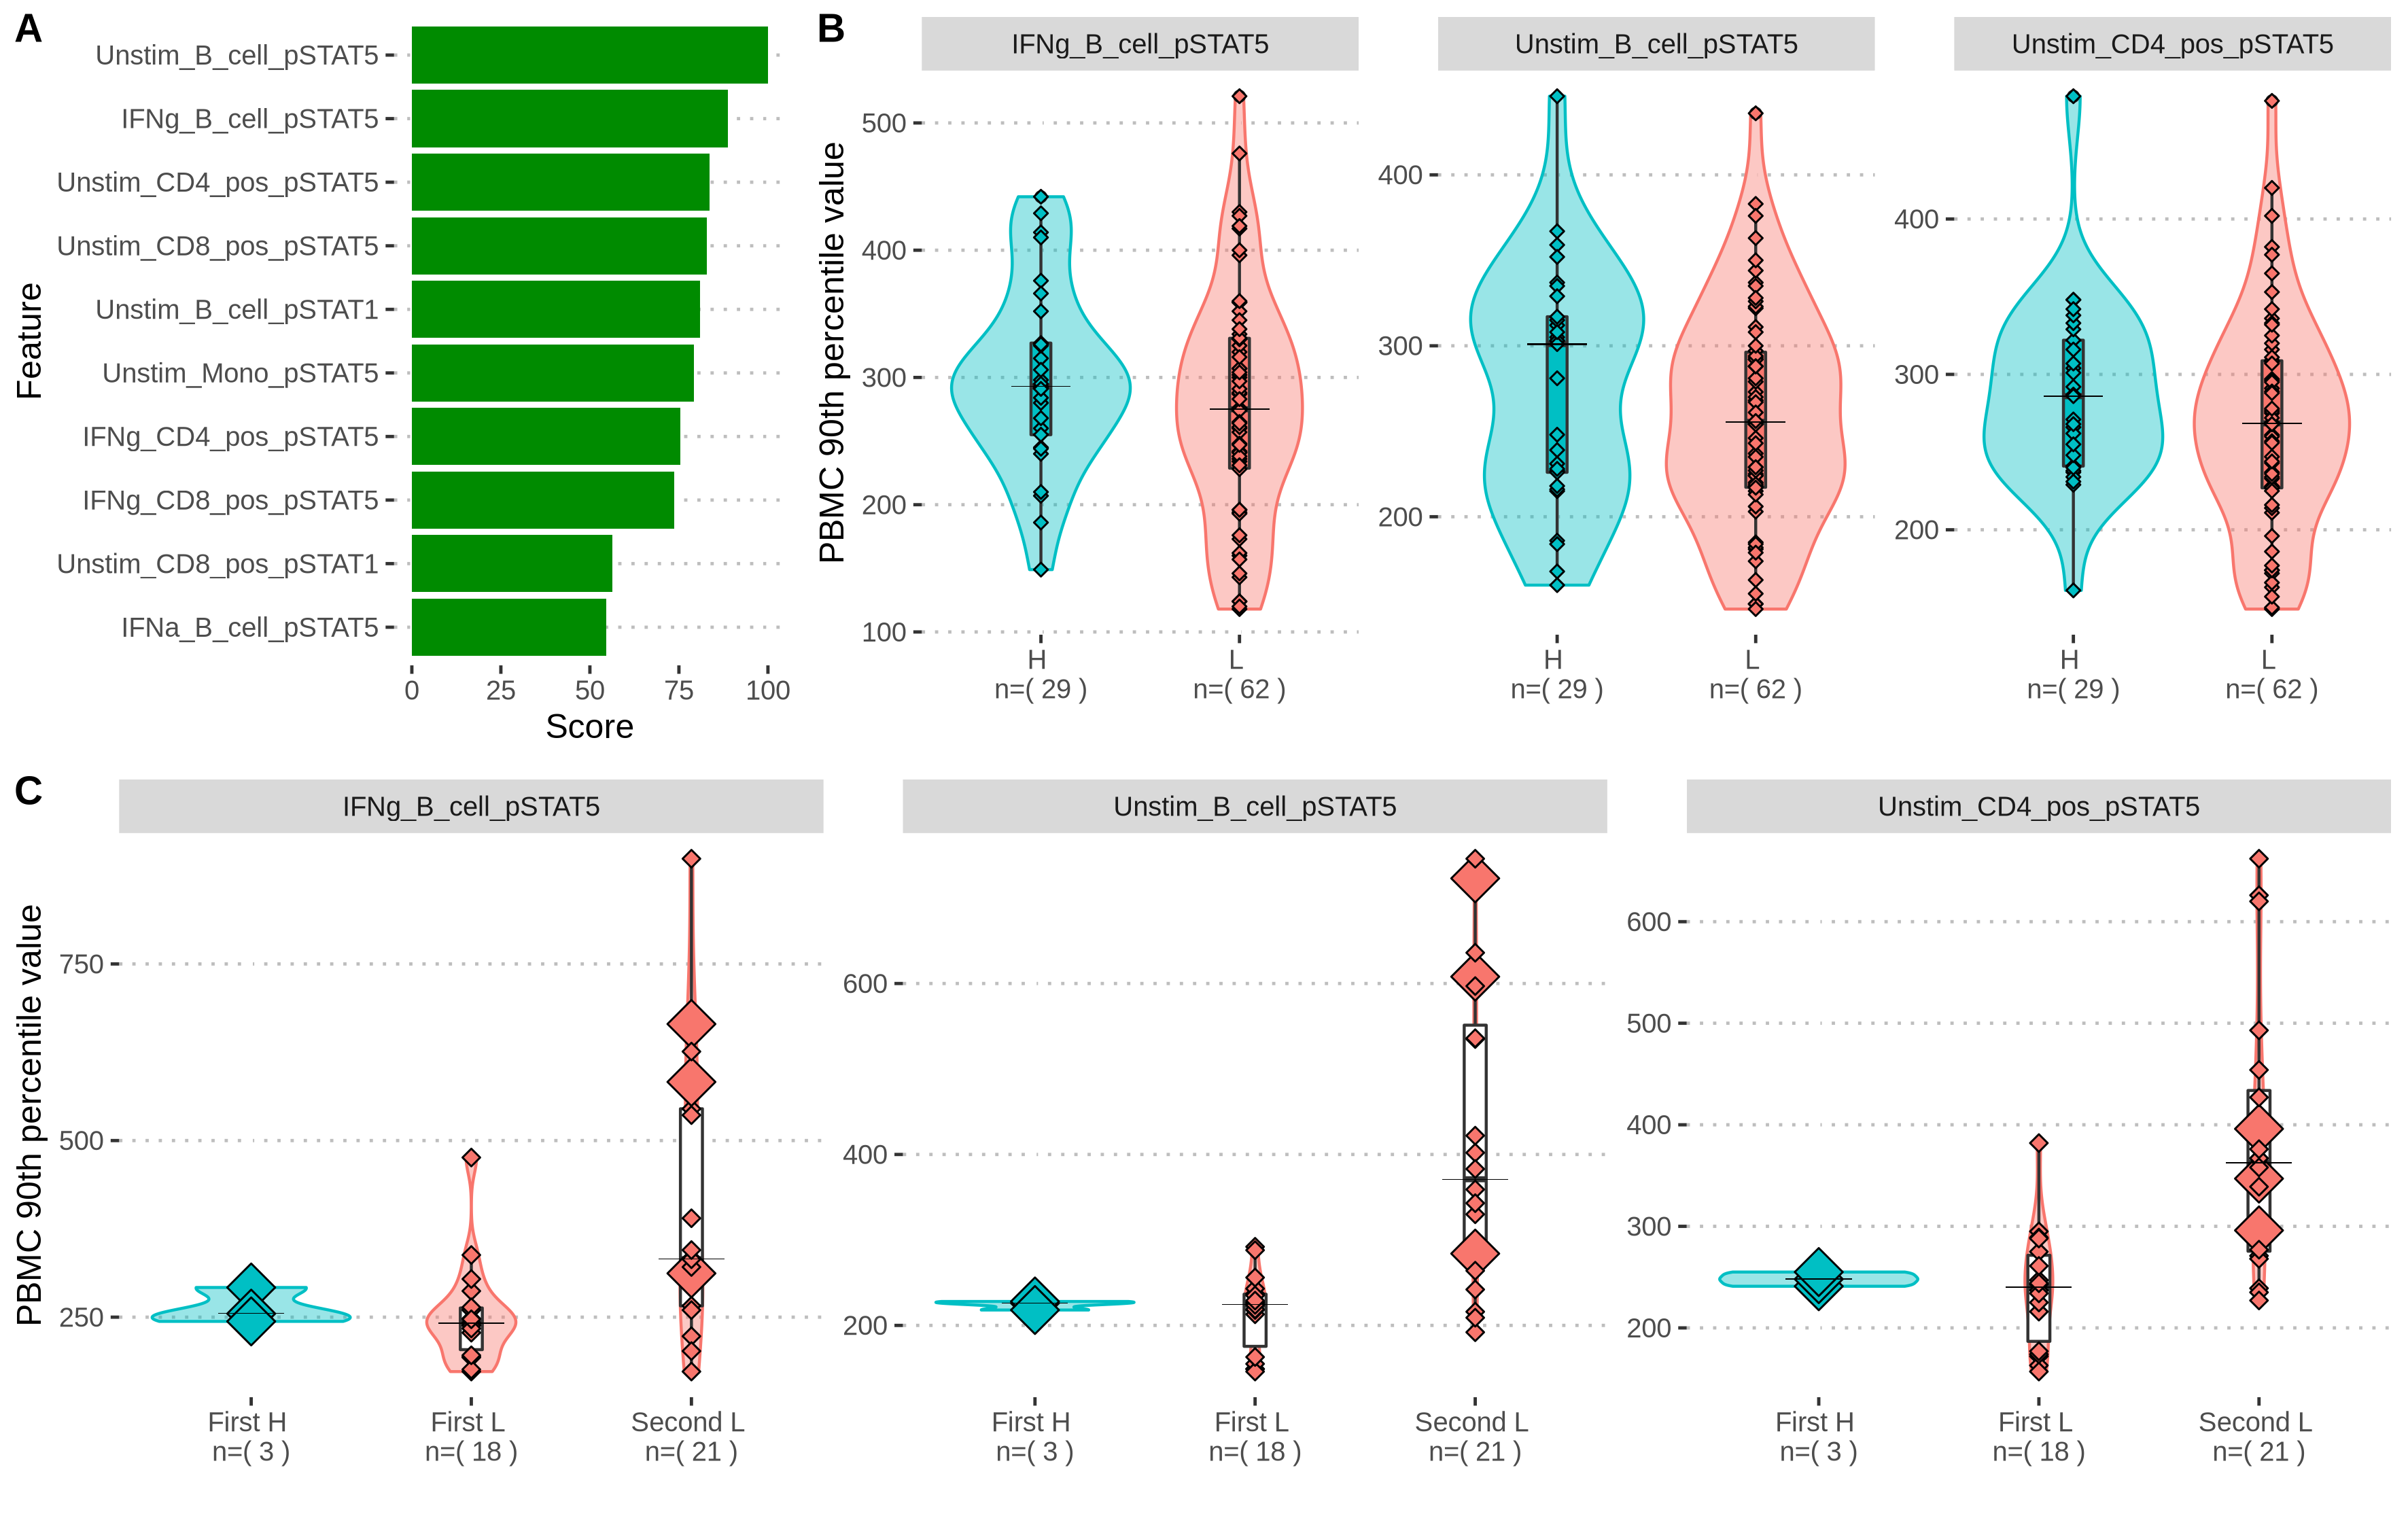
\includegraphics[width=\textwidth]{dataset1_nb_feature_exploration}
    \caption{
        dataset1-nb-feature-exploration
    }\label{fig:dataset1-nb-feature-exploration}
\end{figure}

Firstly, the top ranked feature in dataset 14 was the phosphorylated \gls{bu:stat} transcription factor in unstimulated \gls{bu:bcell}s \autorefsub{fig:dataset1-nb-feature-exploration}{A}.
However, the difference in the value of this feature between the high and low vaccine responders was not found to be significant (at FDR $<$ 0.01) \autorefsub{fig:dataset2-nb-feature-exploration}{B}.
In contrast, the other two features, IFNg stimulated \gls{bu:bcell} phosphorylated \gls{bu:stat} and \gls{bu:cd4pos} phosphorylated STAT5, were found to be significantly greater in the high responder group (FDR $<$ 0.01).
A correlation analysis of all features showed that different \gls{bu:stat} protein formed positively correlated clusters as expected \autoref{fig:cor-dataset1} (p \(<\) 0.0001).
Further, the most important feature had slight negative correlations (pearson's r from -0.2 to -0.5) to a set of stimulated \gls{bu:stat} cell responses (p \(<\) 0.0001 after BH adjustment).
The second most important feature had similar correlations as the first, likely since they are both \gls{bu:bcell} \gls{bu:stat} features.
Lastly, the unstimulated \gls{bu:cd4pos} \gls{bu:stat} phosphorylation also belonged in the same cluster as the previous \gls{bu:bcell} features.
These correlations might indicate an interaction pattern between \gls{bu:stat} and STAT1 phosphorylation in different cell types in response to a vaccine.

\begin{figure}[htpb]
    \centering
    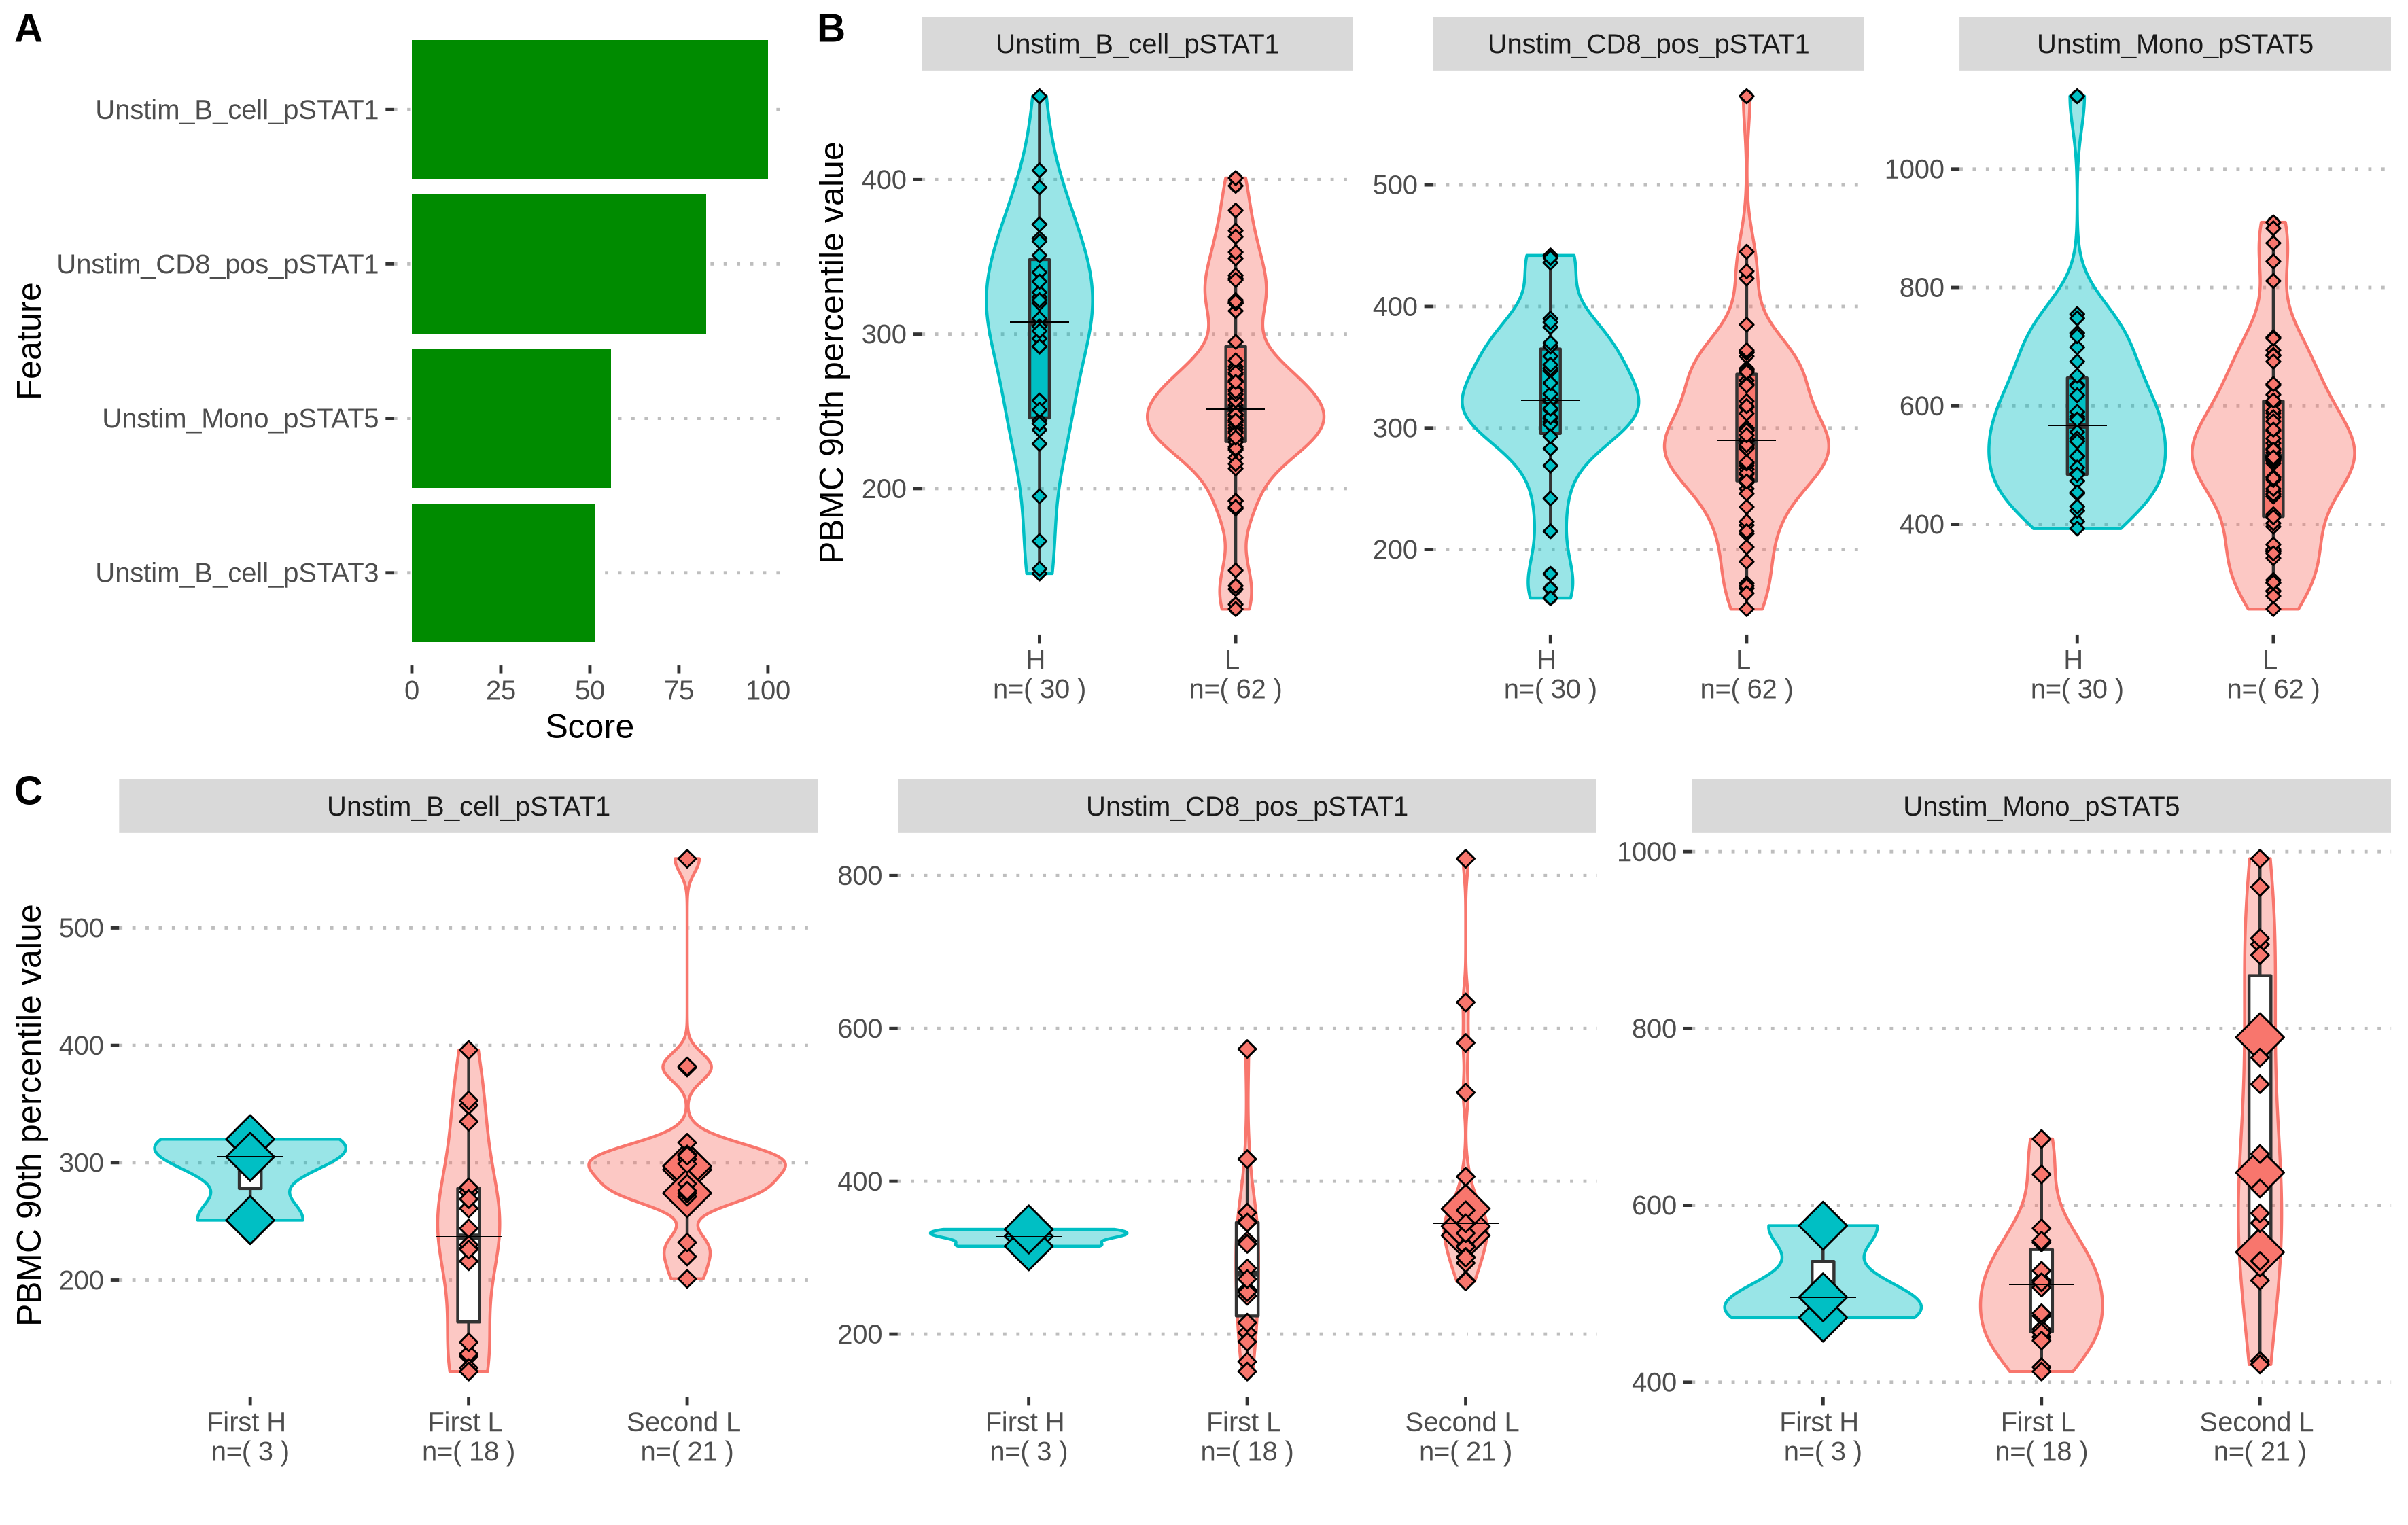
\includegraphics[width=\textwidth]{dataset2_nb_feature_exploration}
    \caption{
        dataset2-nb-feature-exploration
    }\label{fig:dataset2-nb-feature-exploration}
\end{figure}

In dataset 16 there were only four features that had a variable importance score greater than 50 \autorefsub{fig:dataset2-nb-feature-exploration}{A}.
The top two features were phospohorylated \gls{bu:stat} in unstimulated \gls{bu:bcell} and phosphorylated STAT1 in unstimulated \gls{bu:cd8pos}.
However, only the \gls{bu:bcell} feature was found to be significantly greater in the positive class (FDR \(< 0.01\)) \autorefsub{fig:dataset2-nb-feature-exploration}{B}.
The \gls{bu:bcell} \gls{bu:stat} feature correlated positively with both unstimulated \gls{bu:cd4pos} and \gls{bu:cd8pos} STAT1 phosphorylation (pearson's r= 0.7 and 0.4, p \(< 0.001\)), and there were mild negative correlations with interferon gamma stimulated \gls{bu:monocyte} STAT3 and STAT5 phosphorylation (pearson's r= 0.3 and 0.2, p \(< 0.001\)) \autoref{fig:cor-dataset2}.

\subsection{Repeat vaccination effect on identified features}

In the \secondvis of donors in datasets 14 and 16 there were outliers (donors had a value greater than 1000) and nonsensical negative values.
These were left out of visualisations, since outliers made the pattern unclear and the negative values were considered as nonsensical values.

\begin{figure}[htpb]
    \centering
    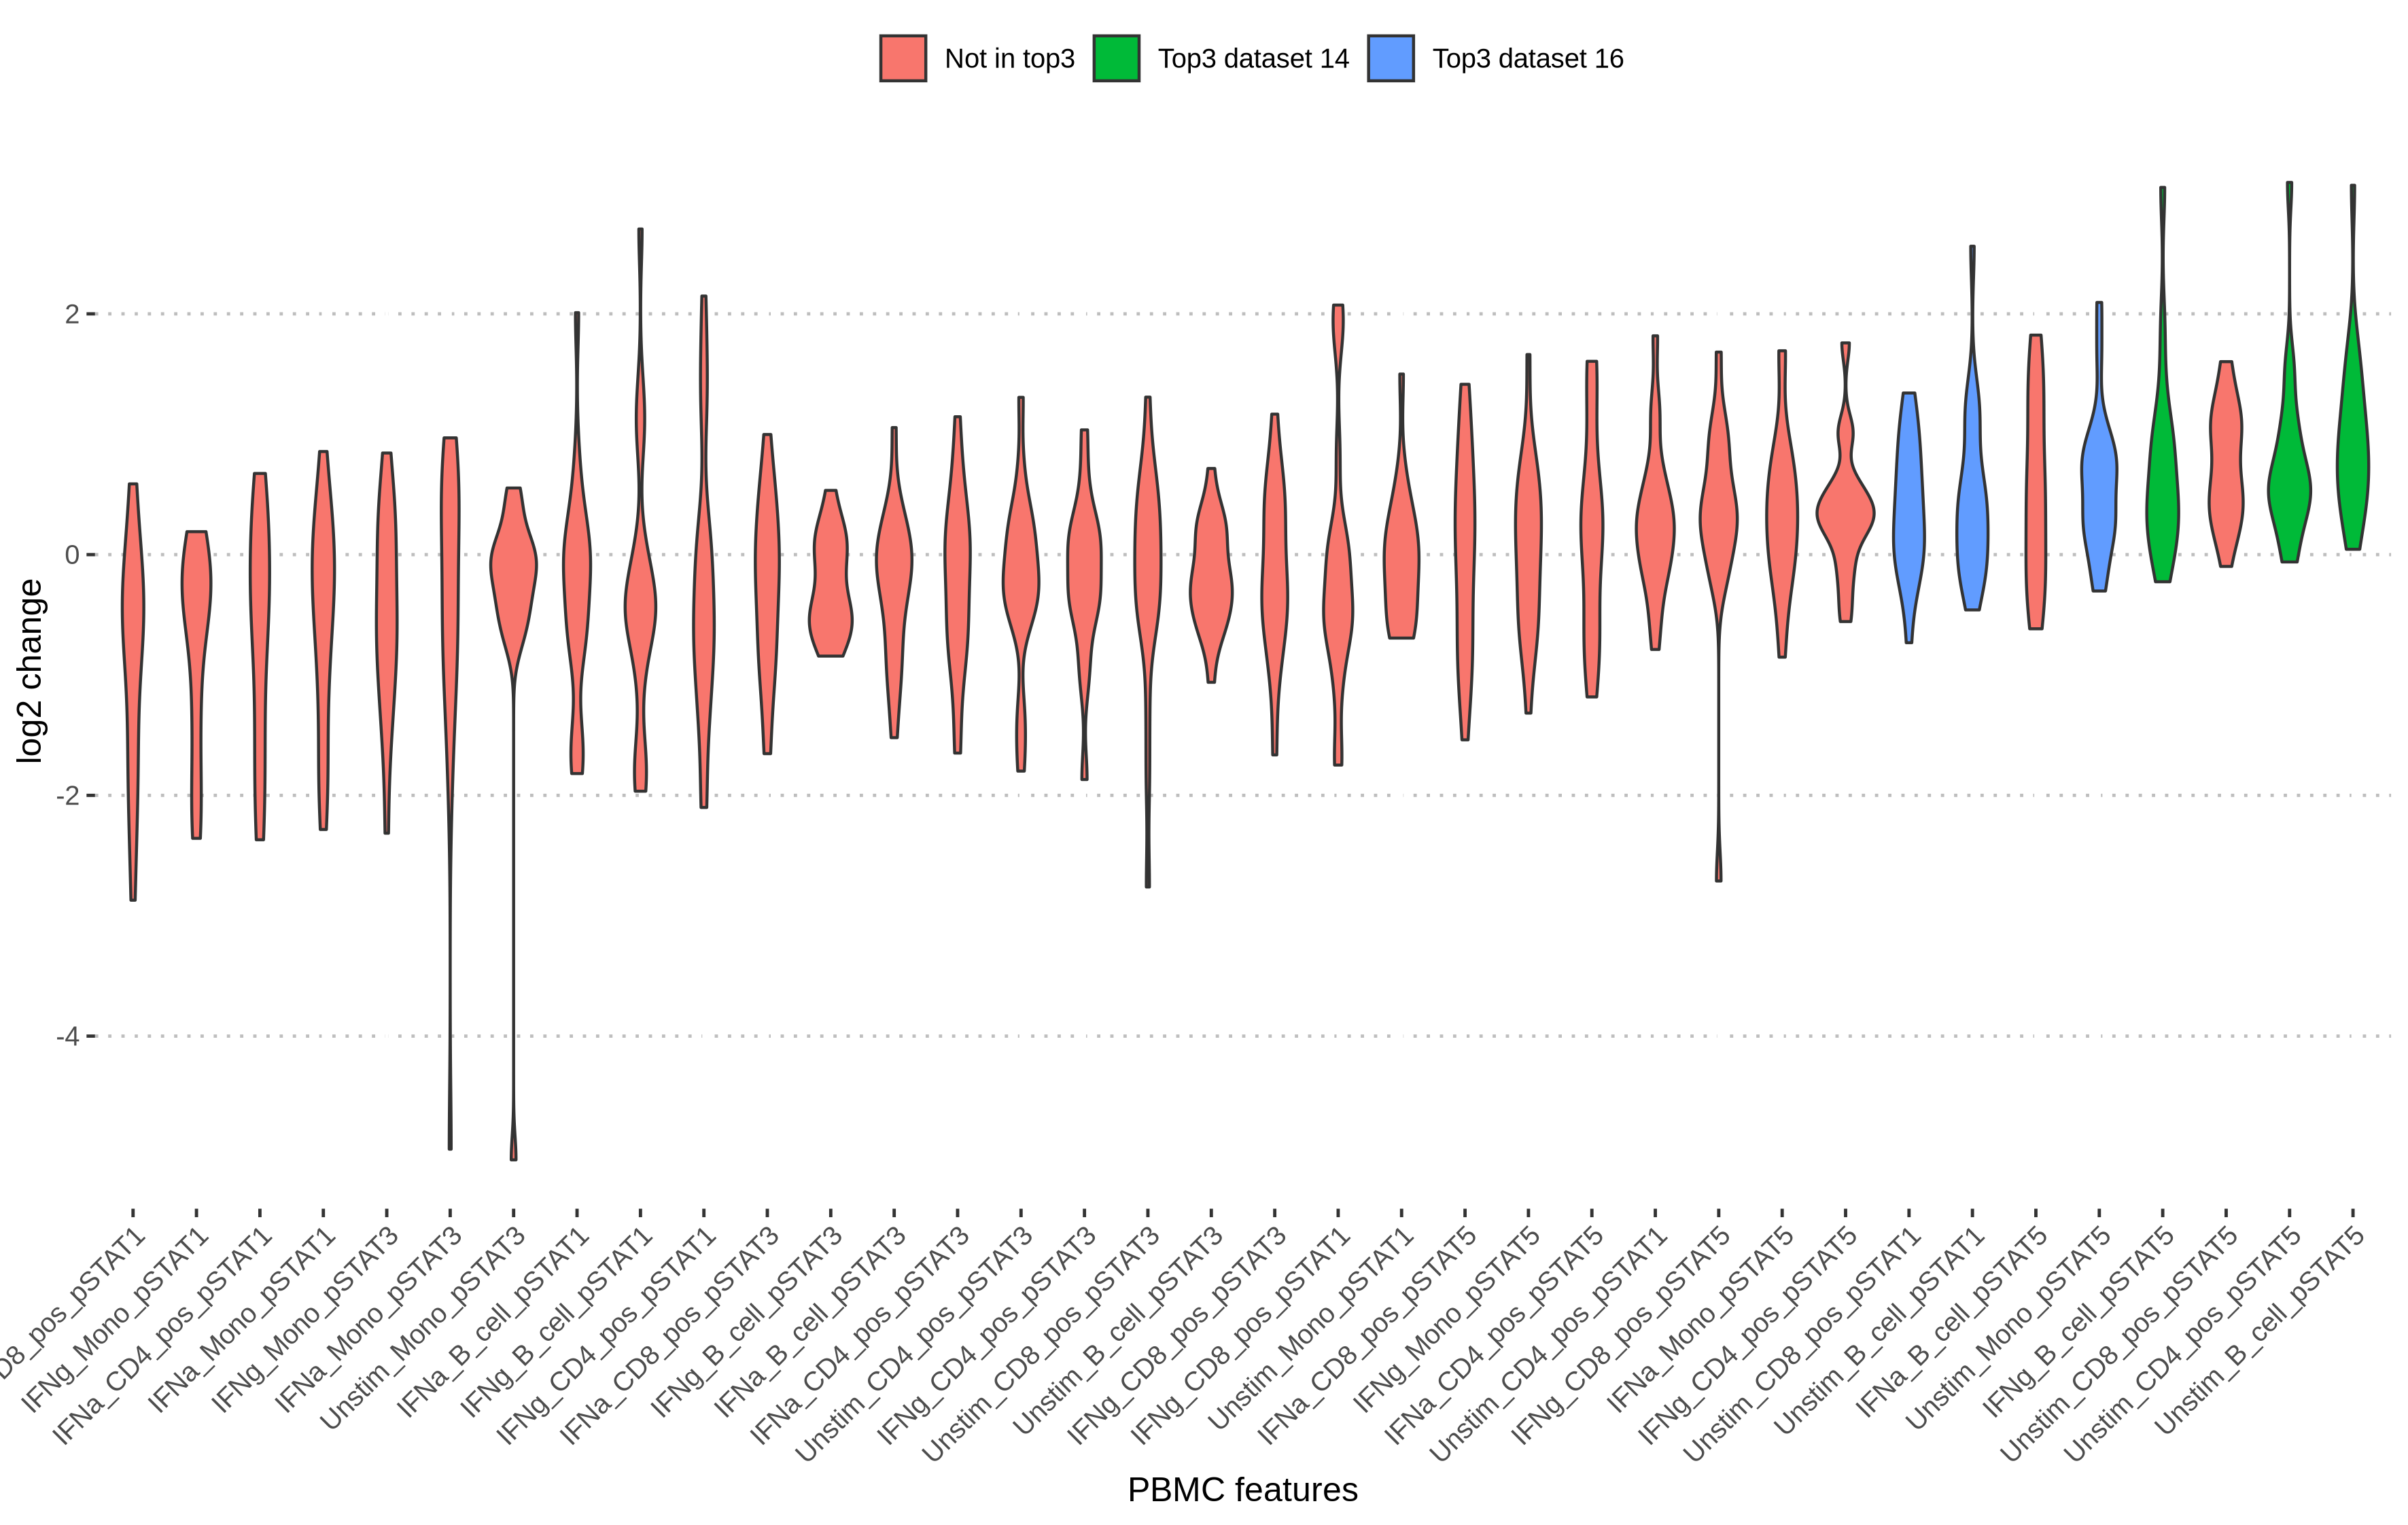
\includegraphics[width=\textwidth]{second_visit_change1}
    \caption{second-visit-change1}
    \label{fig:second-visit-change1}
\end{figure}

To see how a repeat vaccination affects immune cell signaling, the distribution of the top three features of dataset 14 were compared to their distribution when measured in a subsequent influenza season \autorefsub{fig:dataset1-nb-feature-exploration}{C}.
In the 21 donors that had a second measurement of the features in another influenza season that were not left out (outliers and nonsensical values) there was the consistent pattern that the high responders were classified as low responders in their second visit \autorefsub{fig:dataset1-nb-feature-exploration}{C}.
Although, overall the feature values were consistently greater in the \secondvis \autorefsub{fig:dataset1-nb-feature-exploration}{C, enlarged diamonds}.
Thus, vaccination might increase activity in general signaling pathways of PBMC in subsequent influenza seasons, but the classification does not reflect this as increasing influenza antibody response.
One possibility is that the donor was classified as low responder due to a lack of response to one strain of virus in the vaccine administered in the repeat visit, not necessarily to all strains \autoref{fig:classInconsistent}.

To explore the overall change in the features of dataset 14 between the first and subsequent in influenza seasons the distribution of changes for donors were visualised and ordered by mean of log2 change (negative values were removed) \autoref{fig:second-visit-change1}.
The overall trend that appeared was that the unstimulated PBMCs had higher values upon a repeated visit.
And, in general \gls{bu:stat} features increased in value. The values that contributed the most to the model discriminating between high and low responders in the \firstvis also increased the most in a repeat visit.
Although, there are outliers that increased a lot in the subsequent influenza season \autoref{fig:second-visit-change1}.

On dataset 16 two of the top three features had similar distributions to the \firstvis \autorefsub{fig:dataset2-nb-feature-exploration}{C}.
In contrast, unstimulated monocyte cells had higher \gls{bu:stat} phoshporylation in the subsequent influenza season \autorefsub{fig:dataset2-nb-feature-exploration}{C}.
Further, the same three donors that were classified as high responders in the \firstvis and as low responders in the \secondvis as in dataset 14 \autorefsub{fig:dataset1-nb-feature-exploration}{C} had increased monocyte cell \gls{bu:stat} phosphorylation \autorefsub{fig:dataset2-nb-feature-exploration}{C, enlarged diamonds}.
Lastly, the top three features of the model trained on dataset 14 also belonged to those that increased the most between the \firstvis and \secondvis \autoref{fig:second-visit-change1}.

\section{Discussion and conclusion}

In this work we gave a brief introduction into influenza vaccination and how vaccine responses are measured, described the \flup database, and applied a similar data mining method as in \spaper and additionally explored the available repeat vaccination data.
The \flup database made it possible to study vaccine responses by providing a classification of donors into high or low responders based on measured antibody level before and after vaccination.
Further, it combined and preprocessed data from multiple clinical studies in an accessible database format.
This resulted in a wide variety of data on immune cell populations, serum signaling molecules, and cell signaling activity that is suitable for studying immune correlates to vaccine responses using data mining method.
We applied a procedure as described by the authors of \flup in \spaper, wrapper feature selection using multiple models trained on interesting data subsets of \flup. Using this procedure we then explored selected features and how they changed in subsequent influenza seasons.
It was found that \gls{bu:stat} related signaling features correlated with a vaccine response and increased the greatest amount in subsequent influenza seasons.

Initially, the idea was to focus on building accurate predictors of vaccine response by training models including constructed features based on repeat vaccination. However, during the data understanding phase of this project it became clear that \flup contains only complete classifications in the \firstvis.
Instead, the objective was revised to explore the available data on repeat vaccination using models trained on \firstvis data from a selection of clinical studies that received the same vaccine, as done in \spaper.
Overall, during the data understanding phase it became clear that \flup is not suitable for predicting vaccine response with high accuracy, since data is combined from multiple studies and years.
This means using donors/rows from different years and studies creates highly sparse predictors.
Consequently, using \flup data requires selecting small datasets without missing values, this only slightly increases the available example measurements of features by combining data from different studies.
Further, the available data on repeat vaccinations is limited to mostly one clinical study, and in repeat visits there is often no classification making it impossible to train models using repeat vaccination data.

During the data understanding phase we also found that classification is missing in a lot of cases.
Further, we identified an inconsistency in the classification data presented in \flup.
However, this is likely due to the fact that the before and after antibody titer against individual influenza strains in the vaccine is not completely available in the database and not because the classification is incorrect.
Thus to check the classification quality it is necessary to study the raw data and scripts used to generate the database, which is considered out of the scope of this work.

The data preparation and modeling phases included selecting the data that was most suitable for training models and studying repeat vaccinations.
We started with the initial data used in \spaper and also collected repeat vaccination data for the donors in this dataset.
To deal with the sparse data the mulset algorithm was applied to generate twenty small but complete datasets, the three datasets that had the highest amount of donors that received a repeat vaccination were then chosen for modeling and further analysis.
Four models were built all three datasets, but models with fair discriminative ability were built only on dataset 14 and 16.

The features in dataset 14 and 16 were all from the phospho-flow cytometry phosphorylation assay, from them we used the models to identify features correlated with a high vaccine response.
We found that \gls{bu:stat} phosphorylation in immune cells from different lineages was associated with a high vaccine response and was increased in subsequent influenza seasons.
However, further study of this result is considered out of the scope of this work where the focus lies on the application of data science tools.
Instead, we show here that data mining methods described in \spaper can be replicated to answer research questions using complex clinical datasets.

The objectives defined before selecting the data and starting the data preparation and modeling phase of the project were:
\begin{itemize}
        \item What kind of studies can be done using the \flup database?
        \item What immunological factors correlate to a vaccine responses?
        \item What is the effect of repeat vaccination?
\end{itemize}

In summary, we provided insight into which studies can be done using the \flup database by describing the experimental data tables of \flup.
It became clear that \flup is suitable for correlating immunological features with a vaccine response by selecting small complete datasets, but that the possibility of combining large data across years and different studies is limited in \flup.
Additionally, we found that classifications are not available in a great amount of data points limiting the sample size for classification studies.
Further, we identified a group of immune cells from different lineages that had increased phosphorylation activity correlated to vaccine response and found that this increase was present in subsequent influenza seasons.

\section{Materials and methods}

\subsection{Data collection}

By following the guide on the \href{https://github.com/LogIN-/fluprint}{FluPrint Github Repository} the MySQL
server was set up.
All file paths mentioned refer to the github repository of this project which can be found below.

In this work the FluPrint github was first added as a submodule.
This module provides the php scripts to import raw data csv's into the MySQL database.
The operating system and versions of php and MySQL used in this work were OSX "Big Sur" (on Mac Book air 2017), php 7.3.24 (built-in mac version), and MySQL 8.0.23 (homebrew).

In the \href{https://github.com/LogIN-/fluprint}{guide} the dependencies to run
the php import script were installed first. This was also done in this work,
except that the hash-file verification step was skipped.

After the php dependencies were installed the MySQL server was started. By
default homebrew recommends to use the \lstinline{homebrew services [option] [SERVICE]} command to start the MySQL server. However, in this work the server
is started using \lstinline{mysql.server start} which provides a socket that
was symlinked using \lstinline{sudo ln -s /tmp/mysql.sock /var/mysql/mysql.sock}. This was done to prevent an error
(\href{https://stackoverflow.com/questions/15016376/cant-connect-to-local-mysql-server-through-socket-homebrew/18090173}{StackOverflow: cant connect to local mysql server through socket homebrew}) thrown
by the php import scripts. Before the import scripts were run a user was added to the
MySQL server and a database was created \ref{lst:addUser}, the password type had to be \lstinline{mysql_native_password}
(\href{https://stackoverflow.com/questions/62873680/how-to-resolve-sqlstatehy000-2054-the-server-requested-authentication-metho}{how to resolve [SQLSTATEHY000] 2054 the server requested authentication method.}).

\begin{lstlisting}[language=sql, caption=Adding user and database to sql server, label={lst:addUser}]
mysql> CREATE USER 'mike'@'localhost' IDENTIFIED BY ';lkj';
mysql> GRANT ALL PRIVILEGES ON * . * TO 'mike'@'localhost';
mysql> ALTER USER 'mike'@'localhost' IDENTIFIED WITH mysql_native_password BY 'mike';
mysql> CREATE DATABASE fluprint;
\end{lstlisting}

The databasename, the username, and password were added to the
\lstinline{config/configuration.json} of the FlruPrint github module. At this
point the configuration for the php import scripts was finished, and the raw
data downloaded in \lstinline{data/upload} were imported in the MySQL server
using \lstinline{php bin/import.php}.

\subsection{Statistical methods}

\subsubsection{Data selection}

In this work immunological features correlating to a vaccine response were identified using wrapper based feature selection on data from the \flup SQL database.
Suitable datasets without missing values were generated using the \href{https://cran.r-project.org/web/packages/mulset/index.html}{R package mulset}, as described in the data preparation section.
These datasets were split into training and test splits using the createDataPartition function from the R package \href{https://topepo.github.io/caret/}{caret}.
As described in the data preparation and selection sections, datasets were not considered if the test set had less than 10 donors.
Lastly, from the generated datasets the number of donors in the \secondvis was used to choose datasets for further analysis. The \secondvis data was obtained from the database by a query that is avalaible in the github repository of this project.

\subsubsection{Model training, evaluation, exploration}

Standard procedure were used for model training, models were trained only on the training datasets using 10-fold cross-validation that was repeated two times.
The test data was used only as an independent dataset to estimate how much the model overfits on the training data.
Model training itself was done using the \href{https://topepo.github.io/caret/}{caret} R package function train.
Additionally, parameters were chosen based on the highest cross-validated accuracy automatically train function.

Variable importance of the models generated by the \href{https://topepo.github.io/caret/}{caret} package was generated by the function varImp from the same package.
This uses model specific feature contribution statistics and ranks them from most important to not important on a scale from 0 to 100, for example for the naive bayes model it uses the class conditional probabilities of features.

Confusion matrix metrics were generated using the \href{https://cran.r-project.org/web/packages/MLeval/index.html}{MLeval} R package which accepts caret objects and computes metrics in a table format as shown in the model evaluation section.
Additionally, the test AUC was calculated with another R packages called \href{https://cran.r-project.org/web/packages/pROC/pROC.pdf}{pROC}.

Correlation plots of the features from the selected datasets 14 and 16 were made using the R package \href{https://cran.r-project.org/web/packages/corrplot/vignettes/corrplot-intro.html}{corrplot}.

\subsubsection{Significance tests}

To see if features identified by the best classifier trained on datasets 14 and 16 had different distribution in between the two classes the significance analysis of micro arrays (SAM) at a FDR \(<\) 0.01 was used in R.
P values for all correlations shown in the correlation plots below were calculated using an R package, and only correlations with a p-value less than 0.001 were shown.

\subsection{Code and data availability}\label{sec:github}

The code and data belonging to this project can be found in the \href{https://github.com/Vinkage/fluprint_exploration}{github repository}.
The repository contains the directories \lstinline{bussiness_understand}, \lstinline{data_understanding} and \lstinline{data_preparation_modeling} which contain all the \LaTeX source files for what was written during the project.
However, the source files for the final pdf deliverable that is to be graded are in the \lstinline{deliverable} directory.
The directory \lstinline{csv} contains all the flat data files that were generated in this work, \lstinline{queries} contains the SQL source files.
As mentioned above, the import script for constructing the database is added as a submodule called \lstinline{fluprint}.
Other files and directories are data files used in the latex source files.

\printbibliography

\begin{appendices}

    \section{Correlation plots}

\begin{figure}[htpb]
    \centering
    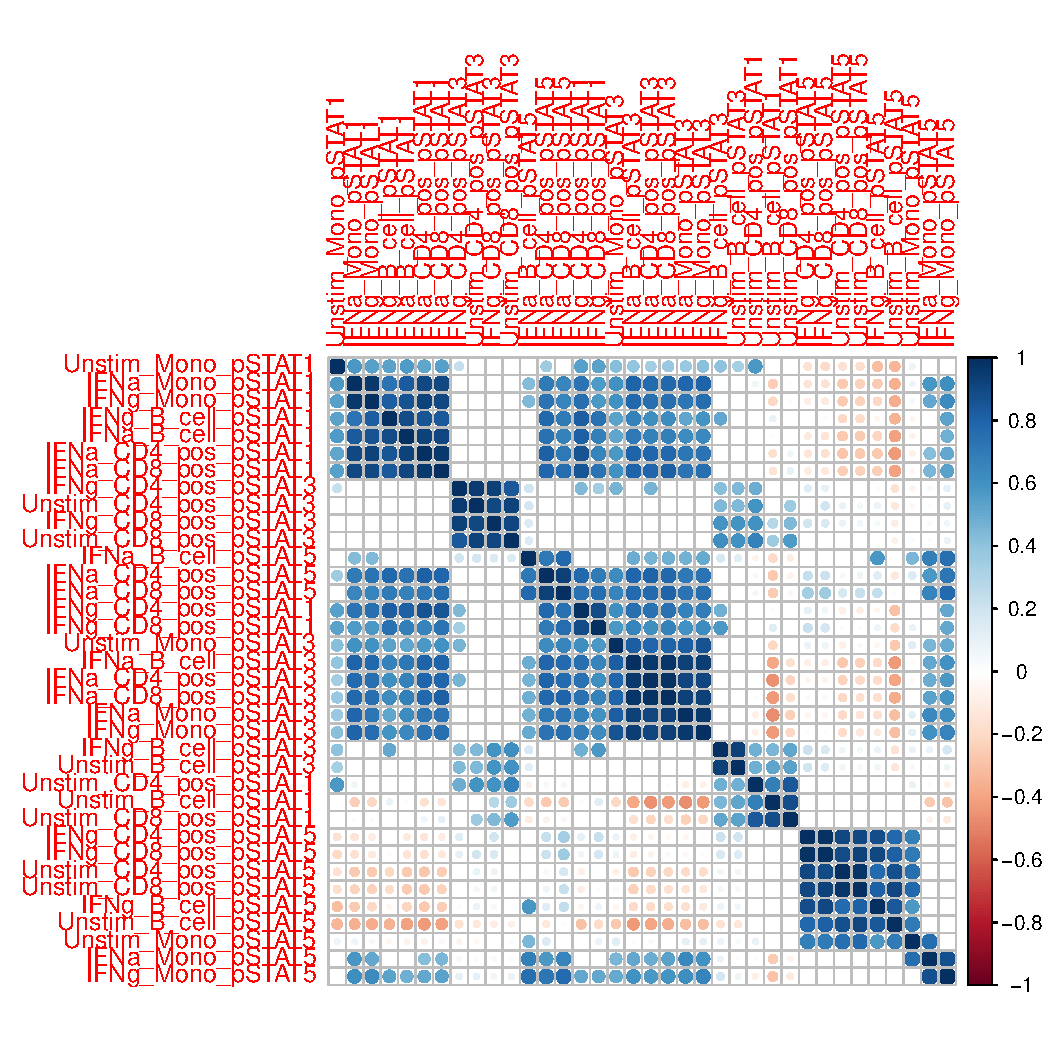
\includegraphics[width=\textwidth]{cor_dataset1}
    \caption{cor-dataset1}
    \label{fig:cor-dataset1}
\end{figure}

\begin{figure}[htpb]
    \centering
    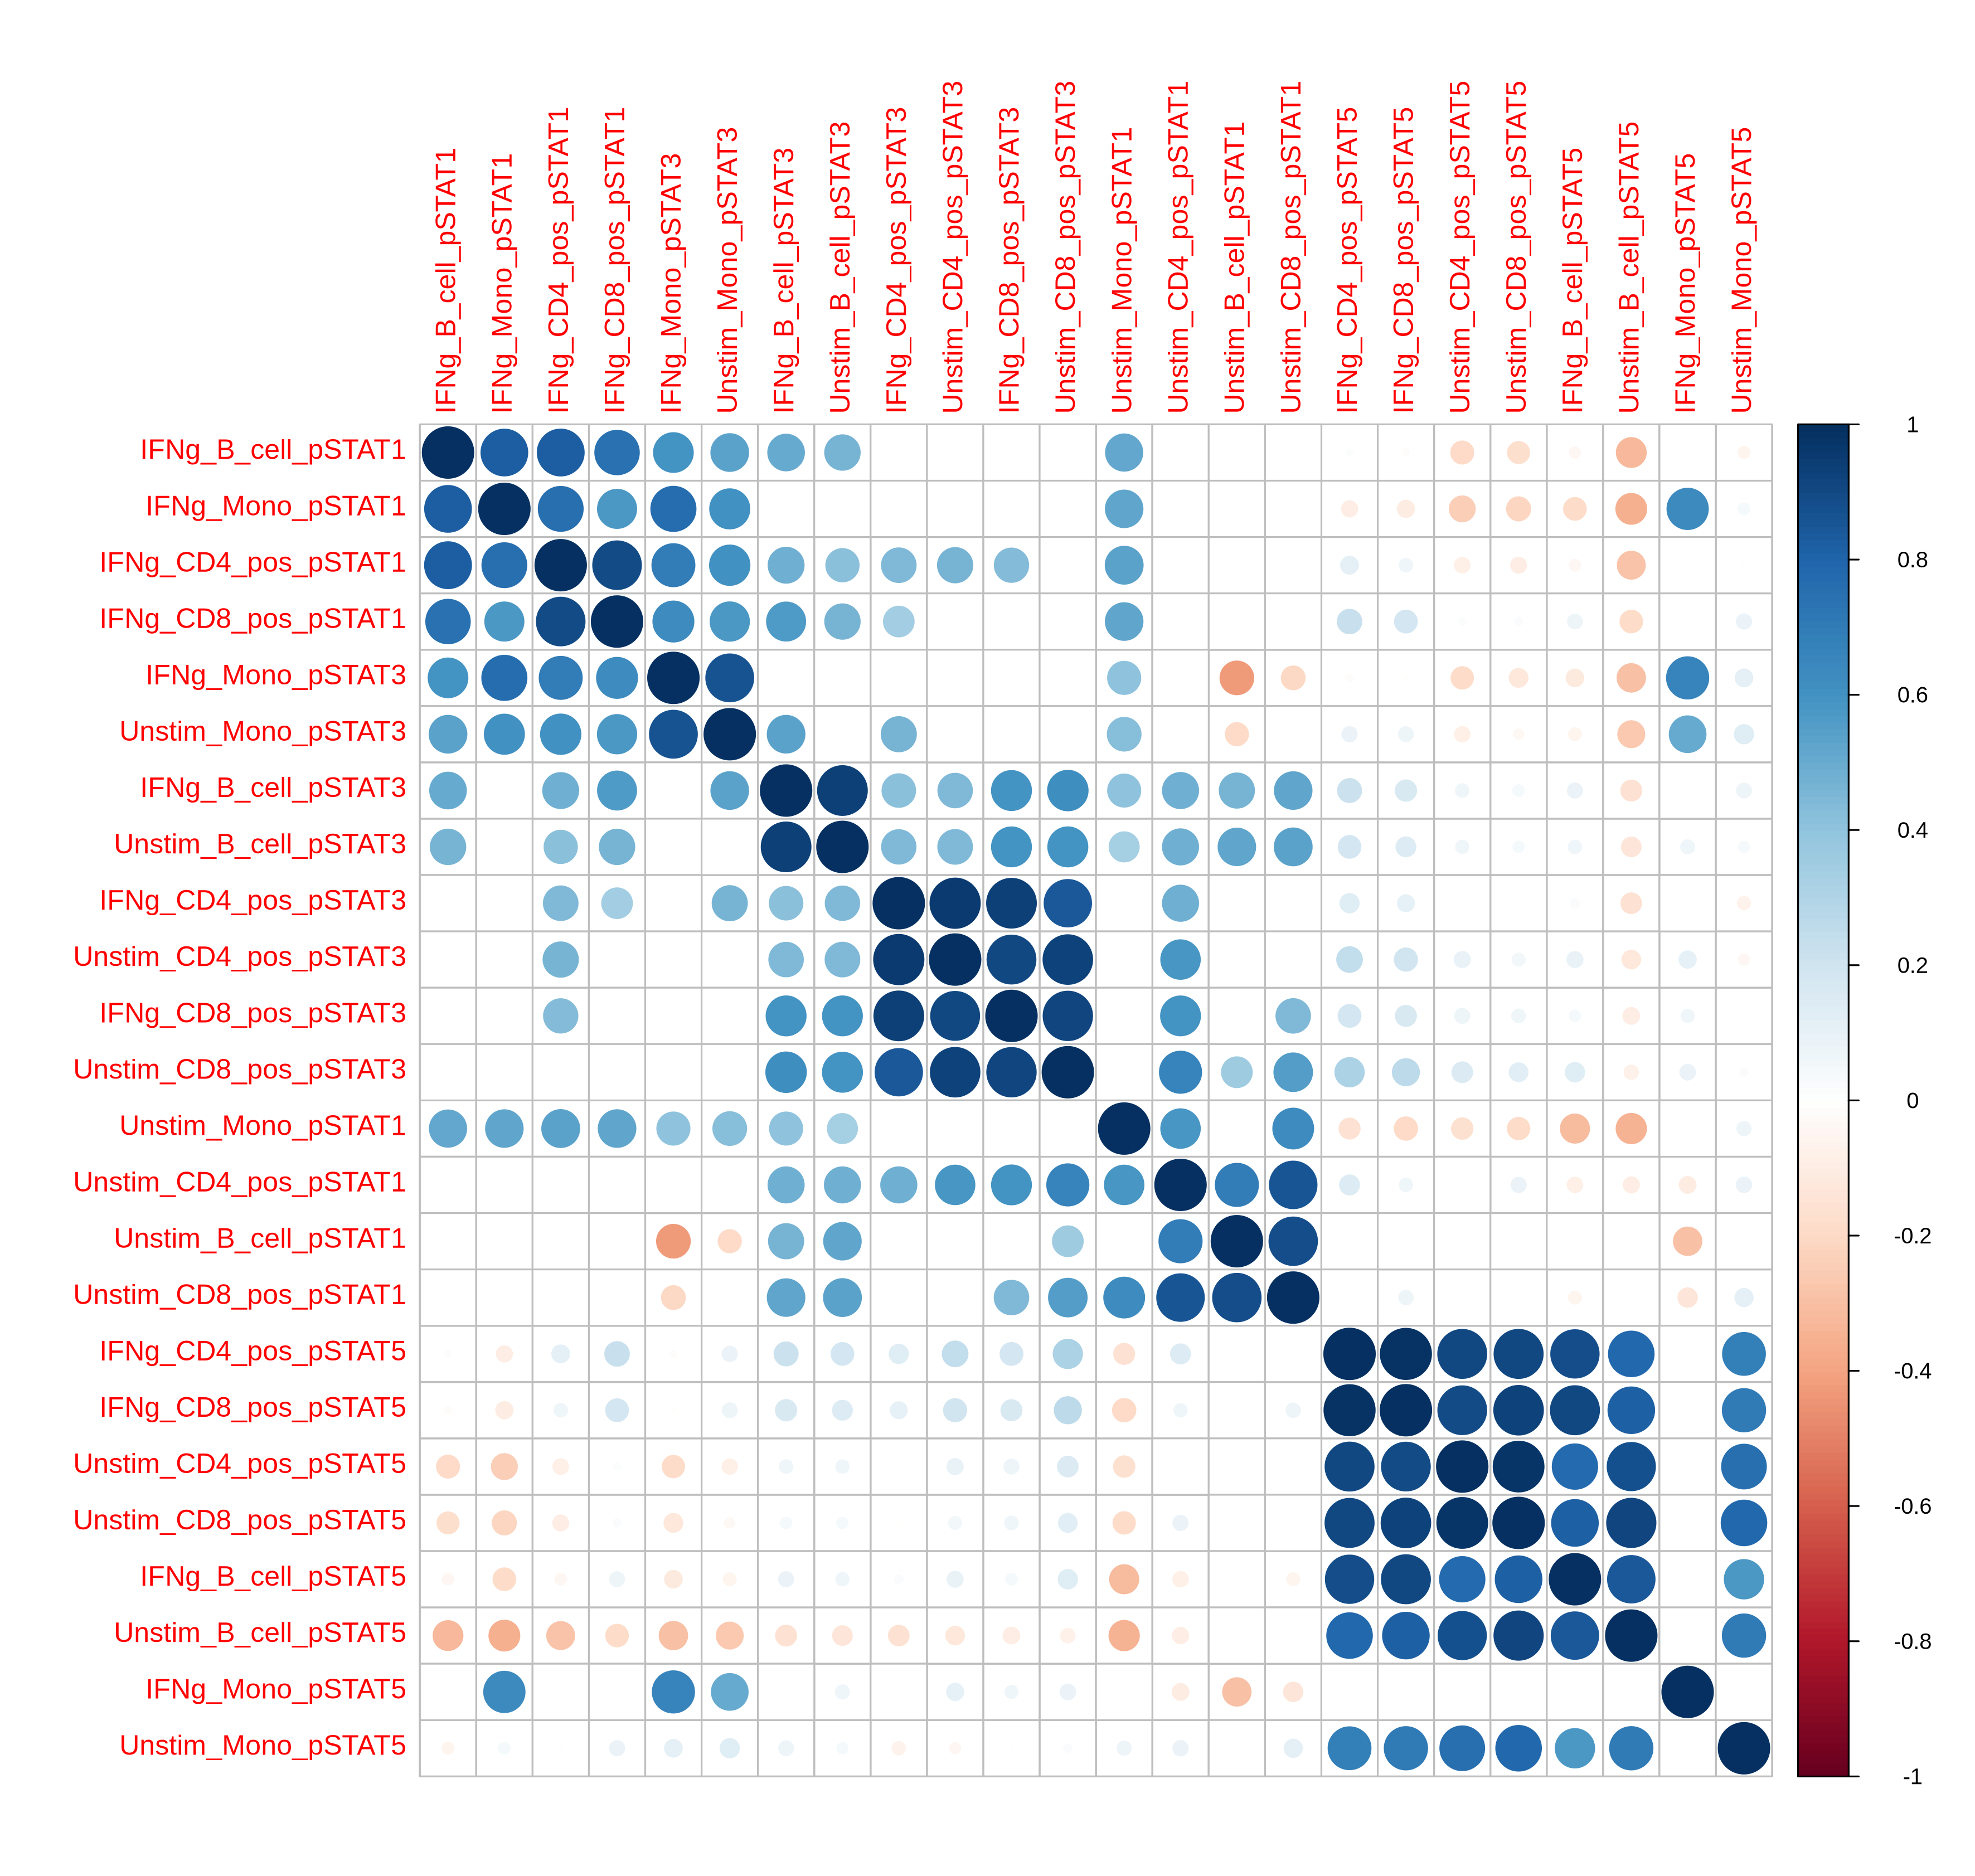
\includegraphics[width=\textwidth]{cor_dataset2}
    \caption{cor-dataset2}
    \label{fig:cor-dataset2}
\end{figure}

    \section{mulset algorithm}

\begin{figure}[htpb]
    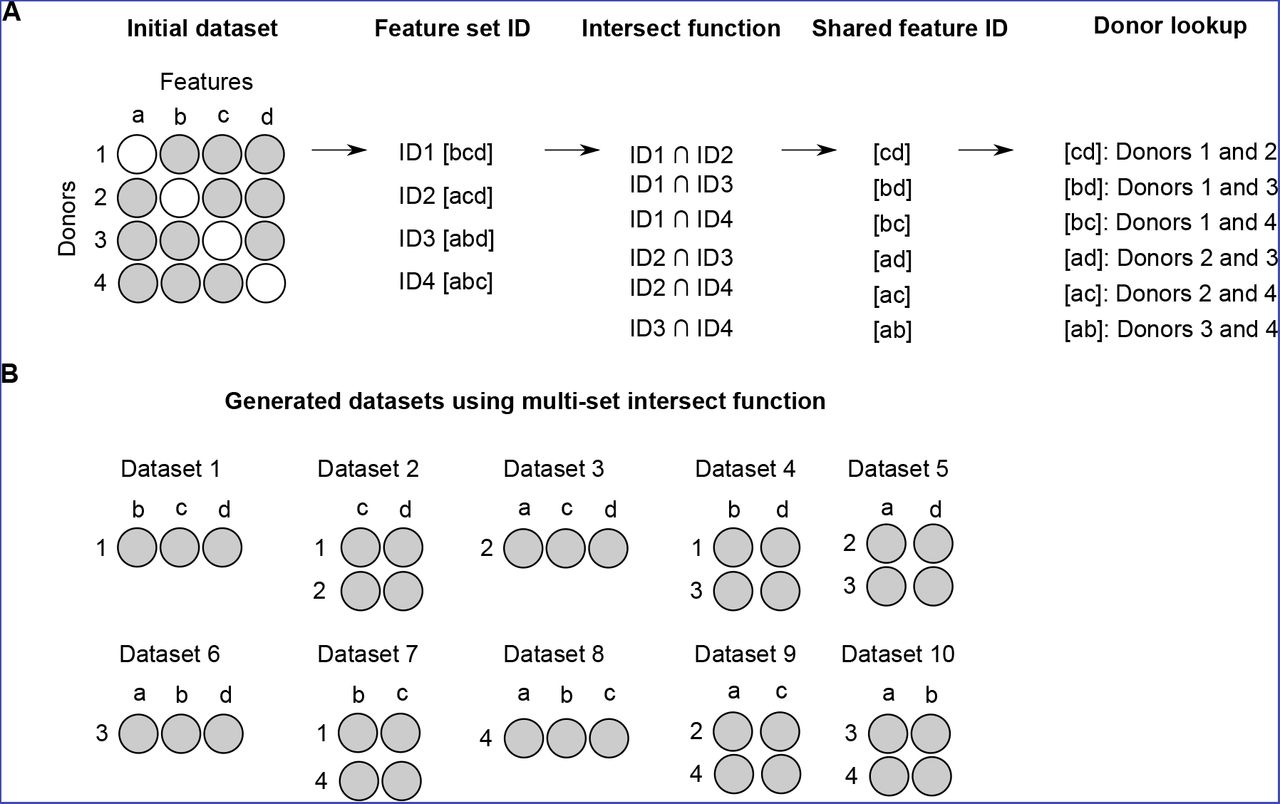
\includegraphics[width=\textwidth]{F2.large}
    \caption{\textbf{taken from original work}}\label{fig:mulsetAlg}
\end{figure}

\begin{table}[htpb]
\addtolength{\leftskip} {-2cm} % increase (absolute) value if needed
\addtolength{\rightskip} {-2cm} % increase (absolute) value if needed
\begin{tabular}{rrrrrlrllrrl}
\toprule{}
donor\_id & study & age & outcome & year & type & hai\_response & name & data\_name & assay & data & dup\\
\midrule{}
285 & 18 & 9.47 & 0 & 2009 & pre & 1 & CD4+ T cells & CD4\_pos\_T\_cells & 13 & 33.8 & TRUE\\
285 & 18 & 9.47 & 0 & 2009 & pre & 1 & CD4+ T cells & CD4\_pos\_T\_cells & 13 & 34.1 & TRUE\\
285 & 18 & 9.47 & 0 & 2009 & pre & 1 & CD4+ T cells & CD4\_pos\_T\_cells & 13 & 34.3 & TRUE\\
285 & 18 & 9.47 & 0 & 2009 & pre & 1 & CD4+ T cells & CD4\_pos\_T\_cells & 13 & 33.0 & TRUE\\
\bottomrule{}
\end{tabular}
    \caption{}\label{tbl:exampleDuplicate}
\end{table}



    \section{Query that generates initial \simon data}
\begin{lstlisting}[language=sql, caption=Query of initial SIMON data, label={lst:QueryTemplate}]
SELECT donors.id                        AS donor_id,
       donor_visits.age                 AS age,
       donor_visits.vaccine_resp        AS outcome,
       experimental_data.name_formatted AS data_name,
       experimental_data.data           AS data
FROM   donors
       LEFT JOIN donor_visits
              ON donors.id = donor_visits.donor_id
                 AND donor_visits.visit_id = 1
       INNER JOIN experimental_data
               ON donor_visits.id = experimental_data.donor_visits_id
                  AND experimental_data.donor_id = donor_visits.donor_id
WHERE  donors.gender IS NOT NULL
       AND donor_visits.vaccine_resp IS NOT NULL
       AND donor_visits.vaccine = 4
ORDER  BY donors.study_donor_id DESC
\end{lstlisting}

    \section{Full description of FluPrint clinical studies}
\fptable{studies_table}{.7}
{Reference table of clinical studies}
{Clinical study ID used (but remapped) in the database, age information,
vaccine type information, and assay data types of clinical studies are in the
rest of the columns.}
{tbl:studiesDesc}


    \section{Remaps used in the \flup}

    \begin{table}[htpb]
        \begin{tabular}{lll}
            \toprule{}
            Vaccine received & Vaccine type ID & Vaccine type name \\
            \midrule{}
            FluMist IIV4 0.2 mL intranasal spray & 1 & Flumist \\
            FluMist Intranasal spray & 1 & Flumist \\
            FluMist Intranasal Spray 2009–2010 & 1 & Flumist \\
            FluMist Intranasal Spray & 1 & Flumist \\
            Flumist & 1 & Flumist \\
            Fluzone Intradermal-IIV3 & 2 & Fluzone Intradermal \\
            Fluzone Intradermal & 2 & Fluzone Intradermal \\
            GSK Fluarix IIV3 single-dose syringe & 3 & Fluarix \\
            Fluzone 0.5 mL IIV4 SD syringe & 4 & Fluzone \\
            Fluzone 0.25 mL IIV4 SD syringe & 5 & Paediatric Fluzone \\
            Fluzone IIV3 multi-dose vial & 4 & Fluzone \\
            Fluzone single-dose syringe & 4 & Fluzone \\
            Fluzone multi-dose vial & 4 & Fluzone \\
            Fluzone single-dose syringe 2009–2010 & 4 & Fluzone \\
            Fluzone high-dose syringe & 6 & High Dose Fluzone \\
            Fluzone 0.5 mL single-dose syringe & 4 & Fluzone \\
            Fluzone 0.25 mL single-dose syringe & 5 & Paediatric Fluzone \\
            Fluzone IIV3 High-Dose SDS & 6 & High Dose Fluzone \\
            Fluzone IIV4 single-dose syringe & 4 & Fluzone \\
            Fluzone High-Dose syringe & 6 & High Dose Fluzone \\
            \bottomrule{}
        \end{tabular}
        \caption{Remaps of vaccine type relevant to to the clinical studies
        reference table \autoref{tbl:studiesDesc}, and the section on the donor
        visits table.}\label{tbl:remapVaccine}
    \end{table}

    \begin{table}[htpb]
        \begin{tabular}{ll}
            \toprule{}
            Original & Remapped \\
            \midrule{}
            No& 0 \\
            Yes& 1 \\
            IIV injection/im& 2 \\
            Doesn’t know/doesn’t remember/na/does not remember& 3 \\
            LAIV4 intranasal/laiv\_std\_intranasal/laiv\_std\_ intranasal/nasal/intranasal& 4 \\
            \bottomrule{}
        \end{tabular}
        \caption{caption}\label{tbl:remapHistory}
    \end{table}

    \begin{table}[htpb]
        \begin{tabular}{ll}
            \toprule{}
            Original & Remapped \\
            \midrule{}
            CMV EBV & 1 \\
            Other immunoassay & 2 \\
            Human Luminex 62–63 plex & 3 \\
            CyTOF phenotyping & 4 \\
            HAI & 5 \\
            Human Luminex 51 plex & 6 \\
            Phospho-flow cytokine stim (PBMC) & 7 \\
            pCyTOF (whole blood) pheno & 9 \\
            pCyTOF (whole blood) phospho & 10 \\
            CBCD & 11 \\
            Human MSD 4 plex & 12 \\
            Lyoplate 1 & 13 \\
            Human MSD 9 plex & 14 \\
            Human Luminex 50 plex & 15 \\
            Other Luminex & 16 \\
            \bottomrule{}
        \end{tabular}
        \caption{caption}\label{tbl:remapAssays}
    \end{table}
\end{appendices}

\end{document}
